%!TEX root = ../thesis.tex
%*******************************************************************************
%****************************** Second Chapter *********************************
%*******************************************************************************

\chapter{Related Work}\label{chap:relwork}

\ifpdf
    \graphicspath{{Chapter3/Figs/Raster/}{Chapter3/Figs/PDF/}{Chapter3/Figs/}}
\else
    \graphicspath{{Chapter3/Figs/Vector/}{Chapter3/Figs/}}
\fi

\section{Introduction}

This chapter discusses background and methods related to 3D shape and pose estimation for articulated subjects. We begin with techniques for correspondence prediction -- a classical method which discusses work focussing on 3D shape and pose estimation for animals. 3D shape and pose estimation for articulated subjects -- primarily animals and humans. We initially focus on skeletal prediction techniques, which output either sets 2D or 3D keypoints. Such techniques are of value to our objective of 3D surface reconstruction, as have been employed in multi-stage pipelines where keypoints are predicted first before a subsequent model fitting stage. The chapter continues with an evaluation of so-called `model-free' techniques, which operate without an explicit template prior.

% Skeletal prediction methods

% Is it a multi-stage approach?
% Does it have a prior?
% 

% Kinect Paper | 

% \section{Point correspondences}
% \section{3D Deformable Model of People and Animals}
% \section{Methods for Single-view Reconstruction}

\section{Predicting point correspondences}

Before delving into methods for 3D reconstruction, it is first necessary to discuss techniques for identifying \emph{point correspondences}. Point correspondences have a long history in computer vision for associating the same real-world location as it is represented by multiple camera views or on a 3D model surface. In a multi-image scenario, determining reliable correspondences between image pairs can be used to greatly reduce the ambiguity when reconstructing 3D scenes from 2D images. Even with only a single image available, correspondences can be predicted between the image and a representative 3D template mesh. This 3D-to-2D correspondence type is important for constraining the class of model fitting algorithms (discussed in depth later) which operate by aligning a 3D template mesh to a given 2D image. Of course, determining point correspondences is made more difficult in the presence of particular nuisance factors. In the case of animal imagery, we must associate points on a non-rigid object with independently moving parts (articulated), deal with frequent self-occlusion in which limbs overlap each other from the perspective of the camera, occlusion caused by environmental factors (e.g. trees, fences, humans etc.), varied and unknown backgrounds and a range of complex lighting conditions (including shadows). Throughout this section, the methods highlighted will be appraised against their suitability in this complex setting.

% https://link.springer.com/article/10.1007/s13735-019-00183-w
% https://arxiv.org/pdf/1603.09114.pdf

\subsection{Relating separate views of the same object/scene}

The first class of techniques focuses on classical approaches for determining corresponding image points taken of precisely the same (and almost always rigid) object. Early techniques focused on stereo~\cite{corres-stereo} or optical flow~\cite{corres-optflow} imagery, and matched image points based on finding regions with similar pixel intensities. Due to the adverse effects caused by changeable environmental factors (e.g. lighting) would have on the appearance of the real-world location when captured in separate images, attention moved towards designing schemes with improved robustness. Improvements were achieved when matching points based on local \emph{mid-level features} such as edges and corners, which have greater invariance to colour changes caused by lighting effects. Typical pipeliens would first identify \emph{interest points} (typically corners~\cite{corner-moravec,corner-harris,corner-susan} or blobs~\cite{sift}), from which local image patches could be compared according to either Squared Sum of Intensity Differences (SSD) or a cross-correlation (CC) scheme. Steady improvements were then made through the design of ever-improving feature descriptors, which encode local image information around points and aim for invariance against common transformations (e.g. viewpoint, rotation and scaling). Progress in this field arguably reached maturity with the advent of SIFT~\cite{sift}, which encodes points according to local histograms of graident orientations and was later speed-up by SURF~\cite{surf} and DAISY~\cite{daisy}. There have been modern attempts to learn sophisticated feature representations using convolutional neural network architectures~\cite{lift, matchnet}, which are shown to offer still further improvement.

The primary aim of these systems is to derive point correspondences between multiple views of the same object, usually as depicted in stereo images or between successive frames of a video. Unfortunately, by matching points based on local geometric features learnt from few image examples, these techniques do not readily extend to identifying correspondences between different instances of the same category. For example, matching SIFT features is likely to result in poor quality correspondences if tested on two dogs of different breeds due to the differing appearance and body geometry. For similar reasons, this class of techniques tend to deteriorate when tested on articulated objects since the object's structure can change and cause self-occlusion between views. The techniques are also known to suffer in scenarios with significant viewpoint changes (e.g. image of the front/back of an animal), since there are few correpsonding points available for matching. Finally, these techniques do not directly offer a method for identifying correspondences between an image and a representative 3D mesh. Although some work exists that extends some of the aforementioned feature descriptors (e.g. 3D-SIFT~\cite{sift-3d}) to 3D, matching typically requires a photorealistic 3D scan of the 2D subject which we cannot assume as input for our problem.

\subsection{Predicting keypoints with a semantic meaning}

This section will explore an alternative class of methods for identifying point correspondences. So far, the approaches described do not detect correspondences with any semantic meaning; in other words, the returned points cannot truly be `named' and there is no guarantee the same points (or even the same number of points) will be identified in different test images. Instead, this section will focus on techniques which predict a set of keypoint locations which are specified in a pre-defined list (for example: nose, tail tip, toe). In general, data-driven machine learning algorithms are used in order to learn an association between image appearance information and semantic keypoint labels. The techniques fall into two general categories: the former set of \emph{supervised techniques} rely on large image datasets manually annotated with keypoint locations, and the latter set of \emph{unsupervised techniques} learn the association through other means. 

\subsubsection{Supervised techniques}

Early work in the supervised prediction of landmarks began through the refinement of object detection methods to predict fine-grained object part labels and eventually progressed to keypoint locations. Perhaps the earliest techniques in this category made use of face part annotations (referred to as fiducial points) to align target faces to improve the face recongition accuracy. Human detection and pose estimation methods progressed from simple bounding box representations~\cite{hog}, to object part prediction~\cite{xxx,xxx}, poselets~\cite{pose-kposelets} and subsequently 2D keypoint localization~\cite{xxx,xxx}. Most commonly, methods aim to predict the location of important 2D human joints (such as the shoulders and wrists) in order to roughly approximate the subject's skeletal pose. For this reason, this task is commonly referred to as \emph{2D human pose estimation}. The earliest techniques represented humans as a graph of parts~\cite{human-rep-parts} and fit shape primitives (e.g. cylinders~\cite{pose-hogg}) to detected edges. Tree-based graphical models known as pictorial structures~\cite{pictorial-structures} were adopted and later made efficient~\cite{pose-felzen}. Improvements were made with models capable of expressing complex relationships betwen joints, such as flexible part mixtures~\cite{yang2013articulated,pose-johnson-mixtureparts}.

Before the popularization of modern deep learning architectures, various methods made use of features computed underneath predicted 2D landmark locations for fine-grained image classification tasks. For this reason, there are limited examples of keypoint datasets for animal categories such as dogs~\cite{liu2012dog} and birds~\cite{WelinderEtal2010}. Chapter 4 of this thesis will discuss StanfordExtra, a new dataset complete with annotated keypoint locations and segmentation masks for 12,000 dog images, encompassing 120 different breeds. At the time of publication, StanfordExtra is the largest annotated animal dataset of its kind. 

% https://arxiv.org/pdf/2012.13392.pdf
Recent works in 2D pose estimation typically employ convolutional neural networks (CNNs) due to the complex feature represenations that can be learnt for joints that, when applied discriminatively, enable accurate recongition. An early example~\cite{pose-embedding} learnt a pose embedding space with a CNN, and employed a nearest neighbour search algorithm to regress a pose. Later, deeper CNN models were used to regress facial point~\cite{pose-face-earlycnn} and full body~\cite{toshev2014deeppose} landmarks. More recent works improve robustness by regressing keypoint confidence maps~\cite{joint-training} rather than 2D keypoints directly, enabling spatial priors to be applied to remove outliers~\cite{cao2018openpose,Pfister15,Pfister14a,Charles16,joint-training,viewpoints-keypoints,pishchulin2016deepcut}. More recent methods are able to directly produce accurate confidence maps through a multi-stage pipeline~\cite{wei2016cpm}. Of particular note are hourglass~\cite{newell2016stacked} (relied upon in this thesis Chapter 3) and multi-level~\cite{sun2019deep,Xiao_2018_ECCV} structures, which combine global reasoning of full-body attributes and of fine-grained details. A related class of methods~\cite{guler2018densepose, taylor2012vitruvian} focus on \emph{dense} human pose estimation, which relate all 2D image pixels to a representative 3D surface of the human body. 

Modern techniques in 2D human pose estimation demonstrate impressive accuracy on in-the-wild datasets, and deal with with parsing multiple subjects in challenging poses and in the presence of various occluders. However, part of what enables these achievements is the prevalance of large 2D keypoint datasets which can be used for training. Further discussion of available 2D keypoint datasets has been left for Chapter 5, in which they are considered in-depth. Further discussion on the history and advances in 2D human pose estimation are comprehensively reviewed in~\cite{2dpose-survey-1, 2dpose-survey-2}.

\subsubsection{Unsupervised learning}

As this thesis focuses on developing methods for animal reconstruction, it is useful to review techniques which operate without large 2D keypoint training datasets, which are scarce for animal subjects. Note that the methods in this section all describe approaches for determining point correspondences between different scenes. Under consideration are methods based on transfer learning, unsupervised learning and methods based on weak-supervision. 

Early correspondence techniques include dense alignment methods including SIFT-flow~\cite{siftflow} which employed optical flow methods to match image using SIFT features, and Bristow et al.~\cite{Bristow2015DenseSC} who demonstrate a method for learning per-pixel semantic correspondences using geometric priors. They also show examples on various animal categories. Recent unsupervised techniques learn \emph{category-specific} semantic priors by employing deep networks on large image collections.

Zhou et al.~\cite{flowweb-efros} demonstrate a method for solving correspondences across an image collection by enforcing cycle consistency. Kanazawa et al.~\cite{kanazawa2016warpnet} introduce WarpNet which predicts a dense 2D deformation field for bird images by learning from synthetic thin-plate spline warps generated on extracted silhouettes. Thewlis et al.~\cite{thewlis-unsup-sphere} apply a similar trick, by ensuring a consistent mapping of warped facial images to a spherical coordinate frame and show results on human and cats. Jakab et al.~\cite{unsup-articulated-objects} show they can estimate 2D human pose without training data data by leverging that between two frames of a simple video sequence, human body shape and texture remains reasonably similar but the pose (including global rotation) varies. They therefore construct an architecture that, given a pair of frames $(I, J)$ defines a network $f$ that given frame $I$ predicts a 2D location vector $y$. The system then combines this vector $y$ with the second frame $J$ and trains a secondary network $g$ to reconstruct the original frame $I$. Due to the limited capacity of $v$, the fact that apart from the pose, most of the information necessary for reconstruction is already available in $J$, the network eventually learns to encode 2D pose coordinates using $v$.

Transfer learning describes a family of methods in which a machine learning model is first \emph{pre-trained} to solve a related task (often making use of secondary dataset with may be larger in size) in order to accumulate knowledge which offers an advantage when solving the original task. DeepLabCut~\cite{mathis2018deeplabcut}, LEAP~\cite{leap-animal-pose} and DeepPoseKit~\cite{graving2019deepposekit} exemplify such techniques, in which existing architectures~\cite{pishchulin2016deepcut,newell2016stacked,densenet,mobilenetv2} are first trained to predict 2D human pose (making use of the large available datasets), and are then repurposed to predict 2D animal keypoints using few (generally 100s) training examples. Cao et al~\cite{animalpose} demonstrate a cross-domain adaptation technique, which transfers knowledge gained from a modestly-sized animal dataset to unseen animal types. There are also dense estimation techniques, which extend DensePose~\cite{guler2018densepose} described above to proximal animal classes~\cite{DenseposeEvo20}, such as chimpanzees, by aligning the geometry between the animal category to humans for which data is plentiful.

% Also under consideration are methods which learn from yet lesser sources of supervision. 

%https://www.robots.ox.ac.uk/~vedaldi/assets/pubs/jakab18unsupervised.pdf
%https://people.csail.mit.edu/celiu/SIFTflow/SIFTflow.pdf
%https://people.eecs.berkeley.edu/~tinghuiz/papers/cvpr15_flow.pdf
%https://www.robots.ox.ac.uk/~vedaldi/assets/pubs/thewlis18modelling.pdf
%https://www.robots.ox.ac.uk/~vedaldi/assets/pubs/thewlis17dense.pdf
%https://www.robots.ox.ac.uk/~vedaldi/assets/pubs/thewlis16fully-trainable.pdf

% https://reader.elsevier.com/reader/sd/pii/S0959438819301151?token=7A13D081FA0EE09BD23EDE5D517D499C7678CD59082C5B225CE01EC8063089BDC30D740FA31FFA6330F7FF6D2FEF2D89
% DeepLabCut: ResNet
% https://www.nature.com/articles/s41592-018-0234-5 (LEAP, StackedHourglass, recently sped up with MobileNet2)
% https://github.com/jgraving/DeepPoseKit
% https://elifesciences.org/articles/47994

% 3D DeepLabCut: https://www.nature.com/articles/s41596-019-0176-0
% AniPose: https://anipose.readthedocs.io/en/latest/
% DeepFly3D: https://elifesciences.org/articles/48571


% TODO: Find out a bit more about sun2019deep, Xiao 2018 etc.
% \section{Image segmentation and object detection}

This section will briefly discuss techniques for extracting binary segmentation masks and object bounding boxes for subjects present in input images.

% \section{3D Skeleton Prediction}





\subsection{More stuff}
There is an extensive body of prior work related to joint position prediction for human subjects. Earlier work used graphical approaches such as pictorial structure models~\cite{andriluka2010monocular,pishchulin2013poselet,johnson2010clustered}, which have since been replaced with deep learning-based methods~\cite{cao2017realtime,bulat2016human}. Few works predict animal joint positions directly owing to the lack of annotated data, although Mathis {\em et al.}~\cite{mathis2018deeplabcut} demonstrate the effectiveness of human pose estimation architectures for restricted animal domains. Our method instead trains on silhouette input, allowing the use of synthetic training imagery. The related task of animal part segmentation~\cite{wang2015joint,wang2015semantic} has seen some progress due to general object part datasets~\cite{chen_cvpr14,zhou2017scene}.

%% Discuss Amazon's system, Novotny's system etc.

\subsection{Applicability to animal categories}
% 2D predictor DeepLabCut 


\section{Modelling articulated subjects}

% Brief introduction and discuss 'non-shape/weak shape' methods. E.g. faces and hands.
% Discuss methods like dolphins or Angjoo birds which start

% face model paper: https://arxiv.org/pdf/1909.01815.pdf

The design of 3D morphable models (3DMMs) has a significant recent history in computer vision research. A 3DMM is a statistical model designed to represent the structure, deformation and apperance space of for a particular object category. Such a model can be constructed for any object category for which a dense point-to-point correspondence can be established between instances. For example, a 3DMM can be designed to represent medium-sized quadrupeds but perhaps not for general animal categories. How, for instance, would one sensibly determine correspondences between a dog and an octupus? 3DMMs have been used extensively as a strong 3D prior to aid various 3D reconstruction algorithms. They are, however, most influential for problems with the most ambiguity: particularly when dealing with articulated objects (e.g. animals or humans), when only a single monocular RGB image is available or when no paired 3D training data is available. 

% cars: 
% ears: https://core.ac.uk/download/pdf/158370989.pdf
% human bodies: http://grail.cs.washington.edu/projects/digital-human/pub/allen03space-submit.pdf
% human bodies: 

Blanz and Vetter~\cite{blanz-vetter} presented the first 3DMM, which expressed a low-dimensional face space space learnt by aligning various face scans. This work, presented over two decades ago, has been recognized with an impact paper award for the continued applications for the ideas presented. Indeed, the approach introduced has found applications far beyond faces~\cite{face-warehouse, basel-old, basel-new}, including for cars~\cite{deformable-cars}, other human body parts including the hands~\cite{Khamis_2015_CVPR} and ears~\cite{deformable-ears}, the human body surface~\cite{anguelov05scape,loper15smpl} and a restricted set of animal categories~\cite{cafm, zuffi2017menagerie}.


This section will cover methods for modelling articulated subjects, focussing primarily methods for human bodies and animals. 


% \subsection{Building 3D morphable models}

%     Of primary concern to this thesis are methods which represent articulated structures, such as human bodies or animals, with a 3D polygon mesh. A polygon mesh $M = (V, T)$ is a collection of vertices, edges bound by vertex pairs, and polygons bound by sequences of edges and vertices~\cite{smith2006vertex}. Although other convex shapes are allowed, this thesis only has need to discuss triangular mesh polygons, which henceforth will be referred to as \emph{triangles}. An example mesh is shown in Figure~\ref{fig:polygon_mesh}. 
            
%         \begin{figure}[H] % Example image
%             \center{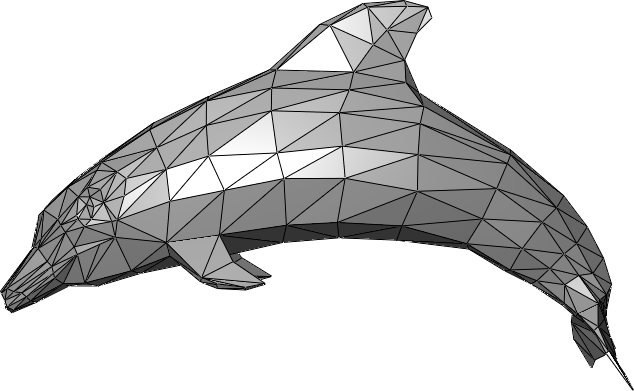
\includegraphics[width=0.5\linewidth]{dolphin_mesh}}
%             \caption{A polygon mesh~\cite{polygon_mesh}.}
%             \label{fig:polygon_mesh}
%         \end{figure}
    
 
%     \subsection{Mesh deformation}
%     The process of adapting a 3D mesh is known as \textit{mesh deformation} and has relevance to a multitude of computer graphics applications, particuarly those in which models are designed to represent dynamic objects. To constrain an optimization function (or simplify the animation process), it is useful to introduce priors that prevent unnatural mesh movement. Two methods for achieving this are discussed:


%         \subsubsection{As Rigid as Possible}
%         As Rigid as Possible (ARAP) surface deformation~\cite{sorkine2007rigid} is a distance function that measures similarity between two meshes with corresponding vertices. For two vertex sets~$V_{1}$ and~$V_{2}$, ARAP minimizes over~$N = |V|$ rotation matrices. Note~$j \sim i$ indicates vertex indices~$j$ adjacent to vertex index~$i$:

%         \begin{equation}
%             D(V_{1}, V_{2}) = \min_{R_{1..N}}\sum_{i=1}^{N}\sum_{j \sim i}|| (V_{1i} - V_{1j}) - R_{i}(V_{2i} - V_{2j}) ||^{2}
%         \end{equation}

%         This distance function can be incorporated into an energy-based optimizer as a regularization function. By considering how small vertex regions overlap, the function can be used to  discourage `unnatural movement', e.g.\ shearing effects, over mesh faces. ARAP regularizers are particularly useful in cases in which there is no prior knowledge of the mesh. Figure~\ref{fig:arap_dino} shows an example of a dinosaur mesh undergoing ARAP deformation, obtained by translating the highlighted yellow vertex.

%         \begin{figure}[H] % Example image
%             \center{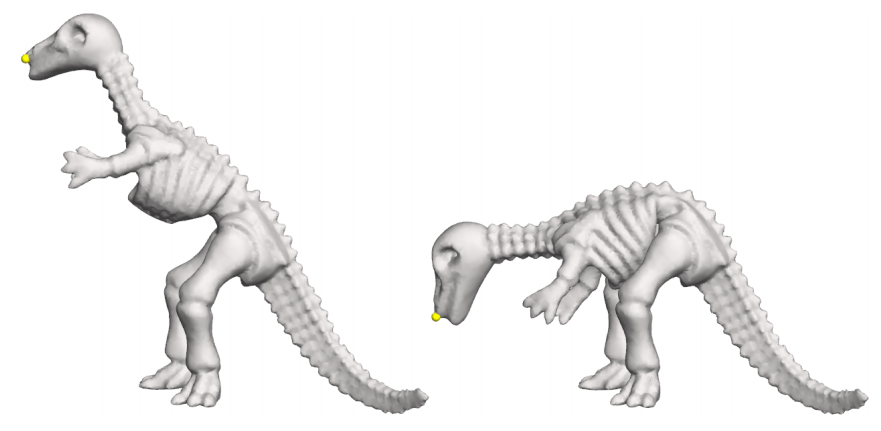
\includegraphics[width=0.35\linewidth]{dino_arap}}
%             \caption{Dinosaur mesh undergoing ARAP deformation, obtained by translating the highlighted yellow vertex. Reprinted from~\cite{sorkine2007rigid}.}
%             \label{fig:arap_dino}
%         \end{figure}


%         \subsubsection{Skeletal Rigging and Linear Blend Skinning}
%         In cases that the mesh shape is known in advance, it is common to follow a process known as \textit{rigging}, in which the mesh is augmented with a hierarchical bone structure. The point at which two bones meet is called a \emph{joint}, and these can be used to define acceptable centres of rotation for mesh deformation. It is possible to describe a distribution of joint configurations, which could be used to constrain the mesh to (in the case of human / animal subjects) anatomically achievable poses. It is also simple to define conceptual `body parts' from a rigged mesh, by considering regions between pairs of joints; for example a lower leg region can be defined between a knee and ankle joint. A simple example of a rigged 2D mesh with joints indicated by green diamonds is shown in Figure~\ref{fig:finger_model}. Note how the mesh surface deforms naturally as the joints are displaced.
        
%         \begin{figure}[H]
%             \centering
%             \begin{subfigure}{0.48\linewidth}
%             \centering
%                 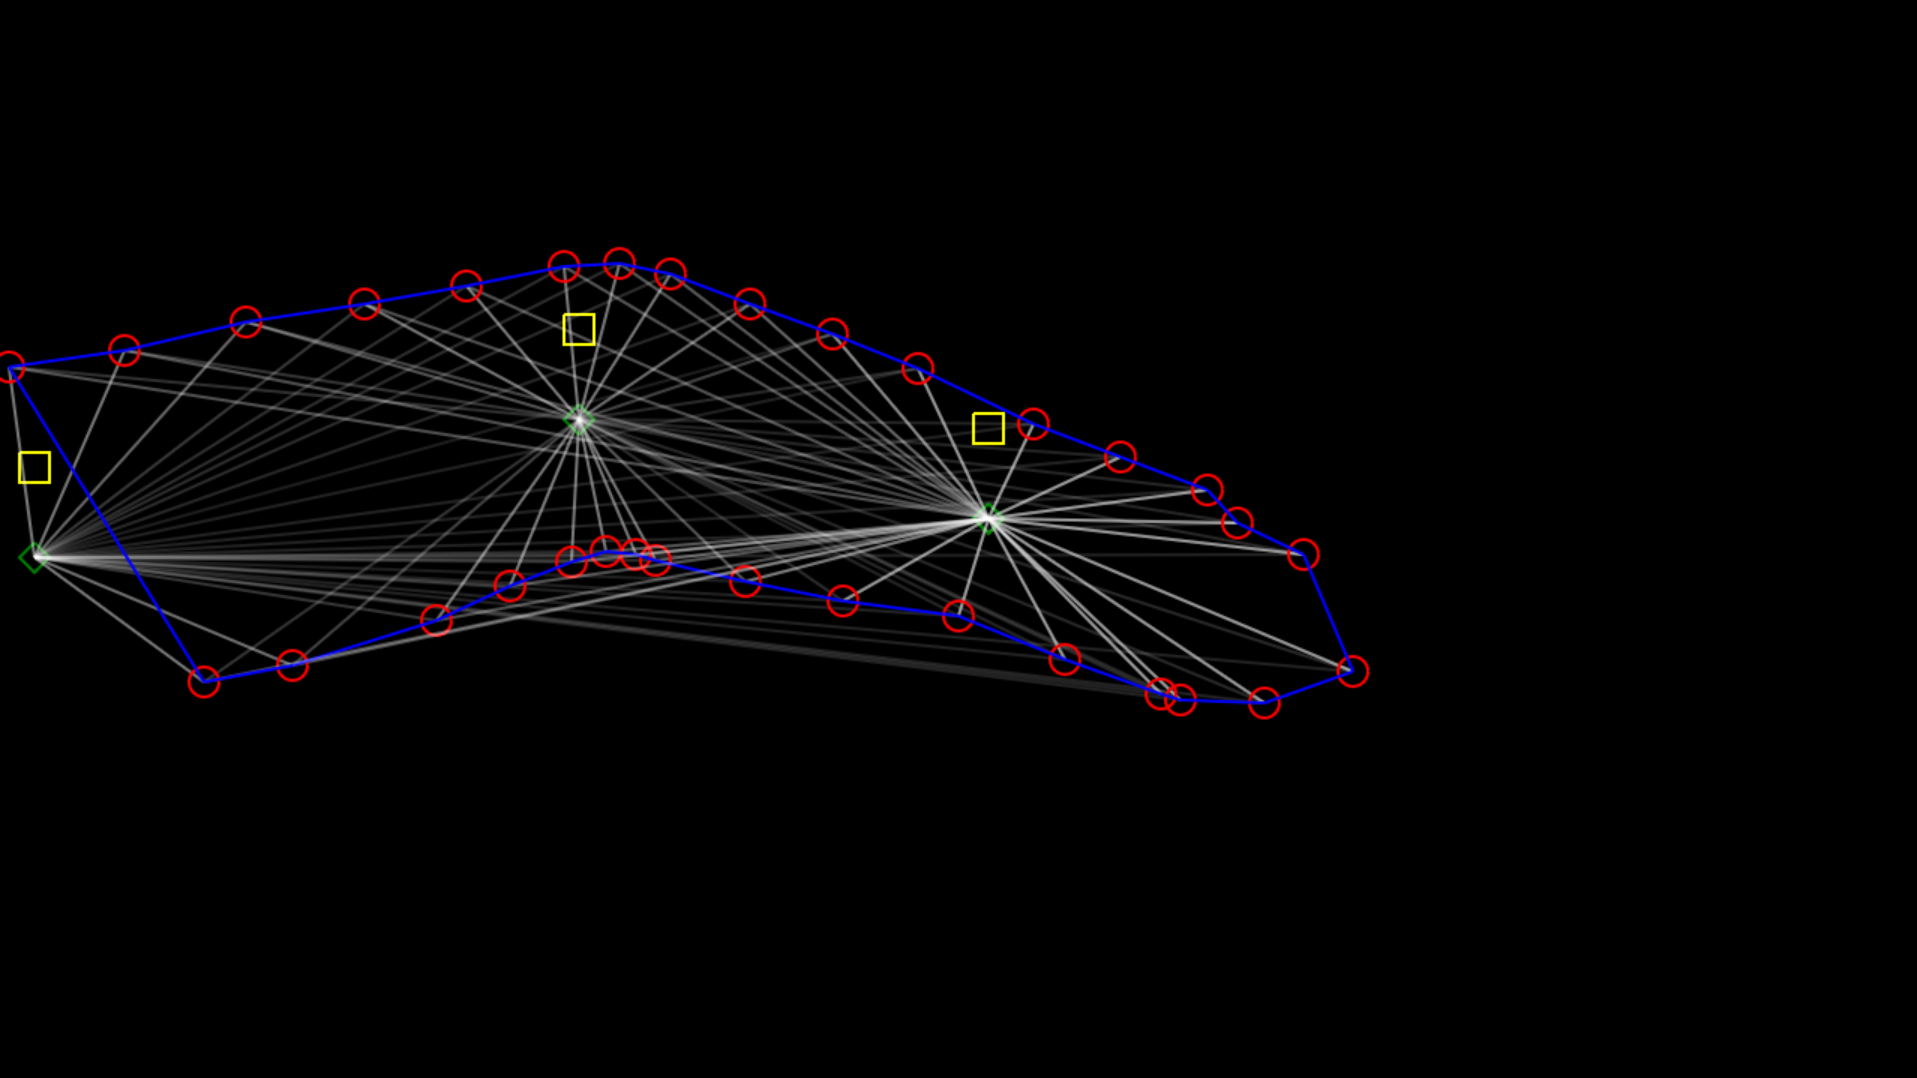
\includegraphics[width=1\linewidth]{finger/finger1}
%                 \caption{Default joint positions.}
%             \end{subfigure}
%             \begin{subfigure}{0.48\linewidth}
%             \centering
%                 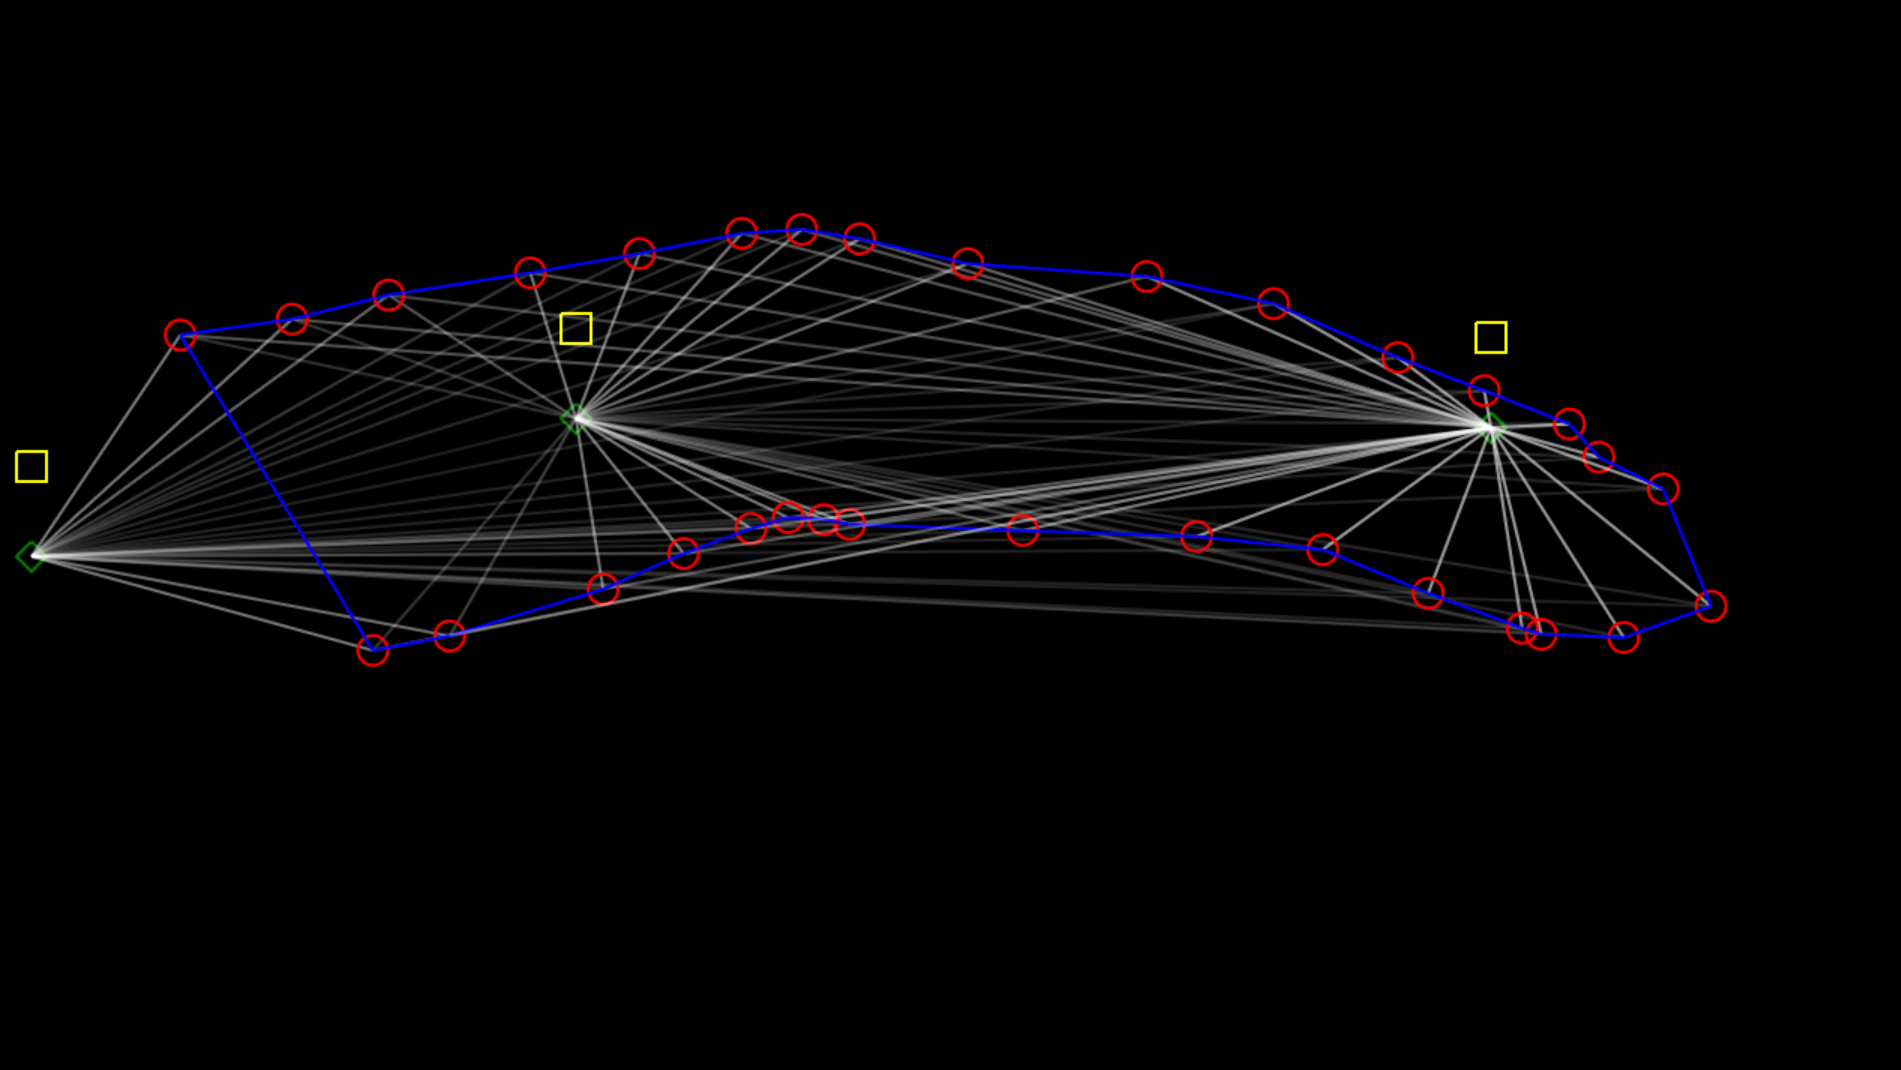
\includegraphics[width=1\linewidth]{finger/finger2}
%                 \caption{Right-most joint displaced.}
%             \end{subfigure}
%             \begin{subfigure}{0.48\linewidth}
%             \centering
%                 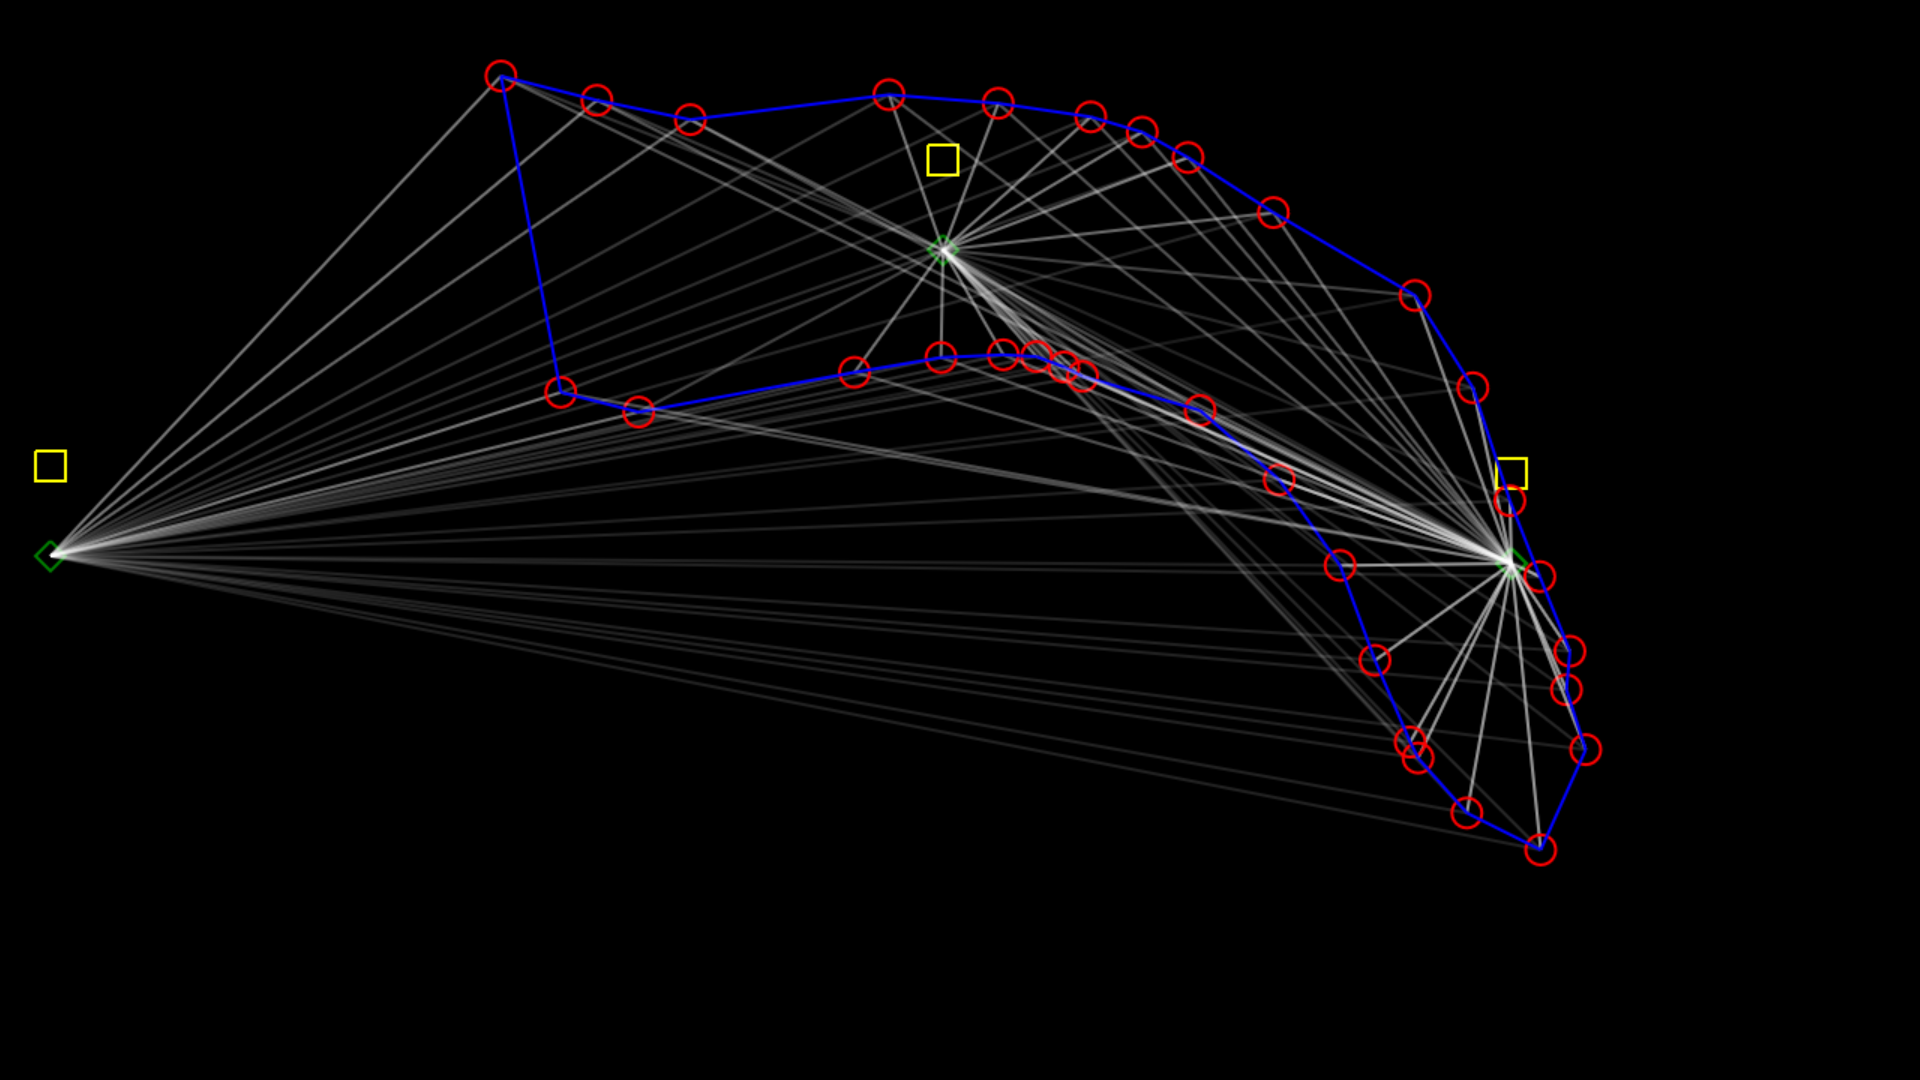
\includegraphics[width=1\linewidth]{finger/finger3}
%                 \caption{Central joint displaced and right-most joint displaced and rotated.}
%             \end{subfigure}%
%             \caption{Web application demonstrating LBS on a 2D finger mesh. Joints are denoted as green diamonds.}
%             \label{fig:finger_model}
%         \end{figure}

%         \clearpage
%         Formally, a skinned mesh consists of a set of rigged vertices $V \subseteq \mathbb{R}^3 \times \mathbb{R}^{|J|}$, a set of faces $F \subseteq V^3$ and joints $J \subseteq R^{3\times3}$. Each vertex $v = (x, s) \in V$ consists of positional coordinate $x \in \mathbb{R}^{3}$ and a weight vector $s \in \mathbb{R}^{|J|}$ which describes the level of influence each joint $j \in J$ has over its movement. Many approaches exist for assigning weights, but perhaps the simplest is to build a vector with entries corresponding to the distance from the vertex to each joint centre. Skinning weight vectors are normalized such that their entries sum to one, and for computational reasons, the number of non-zero elements is typically limited to 2 or 4. The weakness of such models is that artifacts and other unrealistic deformations can occur around the model joints, particularly for meshes that model non-linear structures such as humans. However, the technique is frequently used in computer graphics and game design when a character's shape is known ahead of time.

%         To assist in explanation, Figure \ref{fig:rigged_cylinder} shows skinning weight influences from three joints within a rigged cylinder mesh. Here, $|J| = 3$ and each vertex $v_{i} = (x_{i}, s_{i}) \in V$ has a skinning weight vector $s_{i} \in \mathbb{R}^{3}$. Each model joint is assigned a distinct RGB value, shown separately in (a), (b) and (c), and together in (d) by linearly combining the colours. This linear blend colorization scheme will be frequently used in later sections of this report.

%         \begin{figure}[H]
%             \centering
%             \begin{subfigure}{0.25\linewidth}
%             \centering
%                 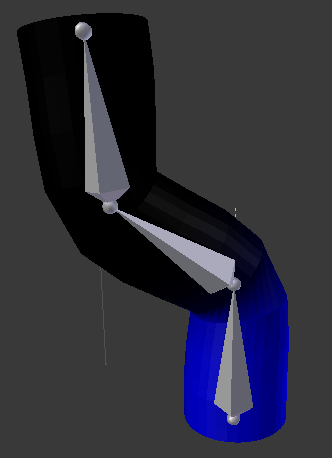
\includegraphics[width=1\linewidth]{wonky_pole/lower_bone}
%                 \caption{Lower joint.}
%             \end{subfigure}%
%             \begin{subfigure}{0.25\linewidth}
%             \centering
%                 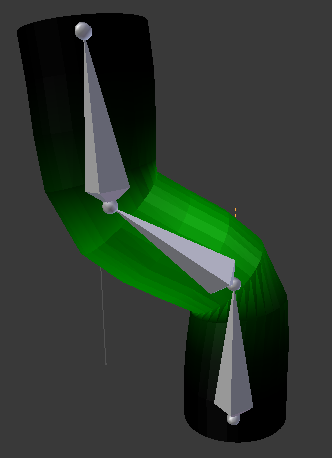
\includegraphics[width=1\linewidth]{wonky_pole/middle_bone}
%                 \caption{Middle joint.}
%             \end{subfigure}%
%             \begin{subfigure}{0.25\linewidth}
%             \centering
%                 
\includegraphics[width=1\linewidth]{wonky_pole/upper_bone}
%                 \caption{Upper joint.}
%             \end{subfigure}%
%             \begin{subfigure}{0.25\linewidth}
%             \centering
%                 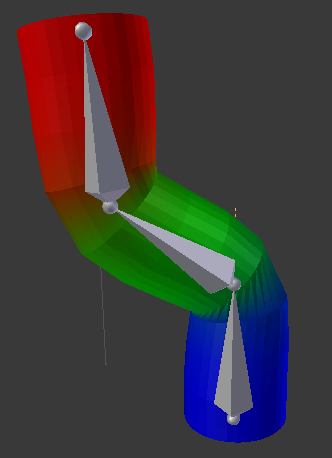
\includegraphics[width=1\linewidth]{wonky_pole/linear_blend}
%                 \caption{Linear blend.}
%             \end{subfigure}%
%             \caption{A rigged cylinder with $|J| = 3$ and where each vertex $v_{i} = (x_{i}, s_{i}) \in V$ has a skinning weight vector $s_{i} \in \mathbb{R}^{3}$.}
%             \label{fig:rigged_cylinder}
%         \end{figure}

%         Figure \ref{fig:rigged_quadruped} shows a more complex rigged quadruped mesh with $|J| = 25$ with skinning weight influences again shown by the linear blend colorization scheme. Again, each joint is assigned a unique RGB value and a vertex's colour is calculated by linearly combining joint colours with skinning weight vectors given by the $\{s_{i}\}$. A triangle's colour is then generated by averaging the colours given for the three surrounding vertices.

%         \begin{figure}[H] % Example image
%             \center{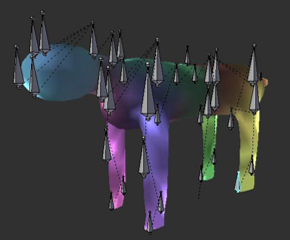
\includegraphics[width=0.5\linewidth]{linear_blend_bold_bones}}
%             \caption{A rigged quadruped with $|J| = 25$ and where each vertex $v_{i} = (x_{i}, s_{i}) \in V$ has a skinning weight vector $s_{i} \in \mathbb{R}^{3}$. Visualization uses the linear blend colorization scheme in which each joint is assigned a unique RGB value.}
%             \label{fig:rigged_quadruped}
%         \end{figure}

%         Once a mesh has been suitably rigged, there are a number of options (e.g. Linear Blend Skinning (LBS), Dual Quaternions~\cite{kavan2007skinning} etc.) for applying a particular mesh deformation. Typically, a user assigns a transformation (in this case comprising a rotation and transformation) to each `joint' and the updated positions $\bar{x_{i}}$ of the remaining vertices $v_{i}$ with original positions $x_{i}$ are then calculated. The original transformation for each joint (i.e. before the deformation) is expressed as a matrix $U_{j}$. The transformation after the deformation has been applied is captured by $D_{j}$. Note that $s_{ij}$ denotes the skinning weight influence of joint~$j \in J$ on vertex $v_{i} \in V$.
        
%         The updated positions $\bar{x_{i}}$ can then be calculated by LBS:

%         \begin{equation}
%             \bar{x_{i}} = \sum_{j=1}^{|J|}s_{ij}D_{j}U_{j}^{-1}x_{i}
%         \end{equation}


% \subsection{Modelling human body parts}

% % Hands, faces etc.


% Given the availability of strong shape and pose priors, articulated hand tracking aptly demonstrates the advantage of model fitting approaches. Again, it is first necessary to decide how the human hand should be parameterized, i.e. what an optimizer should specifically aim to learn. Similar to the case with the full human body, the aim is again to adapt a mesh (although this time of a hand) to reproduce a performance given by a real human hand either in still frames or from an input video sequence. Many modern approaches follow a hand parameterization given by Khamis et al.~\cite{Khamis_2015_CVPR} using a pose vector $\theta \in \mathbb{R}^{28}$ that includes global translation and rotation, one adbuction and three flexion variables for each finger digit, and one abduction and flexion parameter for the wrist and forearm. An example hand tracking result can be seen in Figure~\ref{fig:hand_tracking}. 

\subsection{Constructing 3D morphable models}


% As it relates to modelling rigged articulated objects, it is important to factor deformation into two categories. Firstly \emph{pose} deformations govern the positioning of articulated parts, for example arms and legs. Consequently, parameters for controlling pose will typically vary when reconstructing a sequence exhibiting an articulated subject in motion. \emph{Shape} deformations, however, control the relative lengths and sizes of articulated parts and indeed the global structure. In general, parameters for controlling shape should be invariant to motion and remain consistent for a single individual. 
      
% A frustrating exception to this occurs in the literature discussing face reconstruction. Since models typicaly  since without a define face skeleton, all shape variations are handling face reconstruction, since without a defined face skeleton, all 

% remain consistent In general,  control the relative length and sizing of body parts. In general, only one sizing and length of the model limbs (e.g. arms and legs). typically used to govern the positions of the limbs. are used to govern global and local body proportions (e.g. body part sizes and lengths), and are mostly consistent for a single subject. \emph{Pose deformations} on the other hand are used to govern the positioning of limbs. In order to consolidate various definitions used in the literature, this thesis will define \emph{pose} to be any mesh deformation affected by the movement of an internal skeleton. \emph{Shape} will therefore be any other kind deformation. As an example, then, of most concern to 3D morphable models representing human faces will be \emph{shape} parameters, since face models rarely have an internal skeletal structure. an internal skeleton constitute any deformation change affected by the typically which govern body proportions (e.g. body part sizes, lengths) and \emph{pose deformation} which governs the positioning of limbs. Of course, a typical image of a human or animal will comprise 

3D deformable models are typically represented by a polygon mesh. A polygon mesh $M = (V, T)$ is a collection of vertices, edges bound by vertex pairs, and polygons bound by sequences of edges and vertices~\cite{smith2006vertex}. Although other convex shapes are allowed, this thesis only has need to discuss triangular mesh polygons, which henceforth will be referred to as \emph{triangles}. An example mesh is shown in Figure~\ref{fig:polygon_mesh}. 

\begin{figure}[H] % Example image
    \center{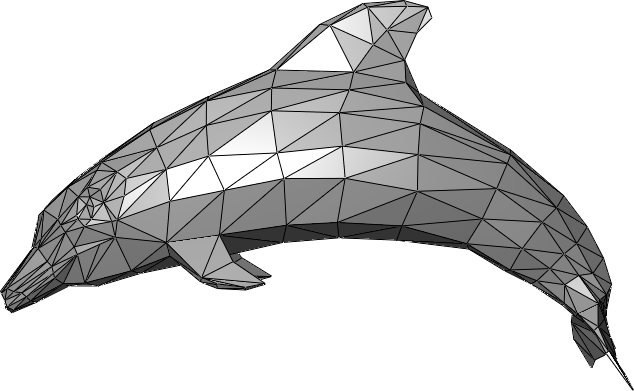
\includegraphics[width=0.5\linewidth]{dolphin_mesh}}
    \caption{A polygon mesh~\cite{polygon_mesh}.}
    \label{fig:polygon_mesh}
\end{figure}

A 3D morphable model can then be constructed by deforming a template mesh $M$ on $n$-vertices to a set of 3D training examples. Generally, this optimization will have a significant degrees of freedom so it is necesssary to employ techniques for regularization. One such regularizer is known as the \emph{As Rigid as Possible} scheme: 

\subsubsection{As Rigid as Possible}
As Rigid as Possible (ARAP) surface deformation~\cite{sorkine2007rigid} is a distance function that measures similarity between two meshes with corresponding vertices. For two vertex sets~$V_{1}$ and~$V_{2}$, ARAP minimizes over~$N = |V|$ rotation matrices. Note~$j \sim i$ indicates vertex indices~$j$ adjacent to vertex index~$i$:

\begin{equation}
    D(V_{1}, V_{2}) = \min_{R_{1..N}}\sum_{i=1}^{N}\sum_{j \sim i}|| (V_{1i} - V_{1j}) - R_{i}(V_{2i} - V_{2j}) ||^{2}
\end{equation}

This distance function can be incorporated into an energy-based optimizer as a regularization function. By considering how small vertex regions overlap, the function can be used to  discourage `unnatural movement', e.g.\ shearing effects, over mesh faces. ARAP regularizers are particularly useful in cases in which there is no prior knowledge of the mesh. Figure~\ref{fig:arap_dino} shows an example of a dinosaur mesh undergoing ARAP deformation, obtained by translating the highlighted yellow vertex.

\begin{figure}[H] % Example image
    \center{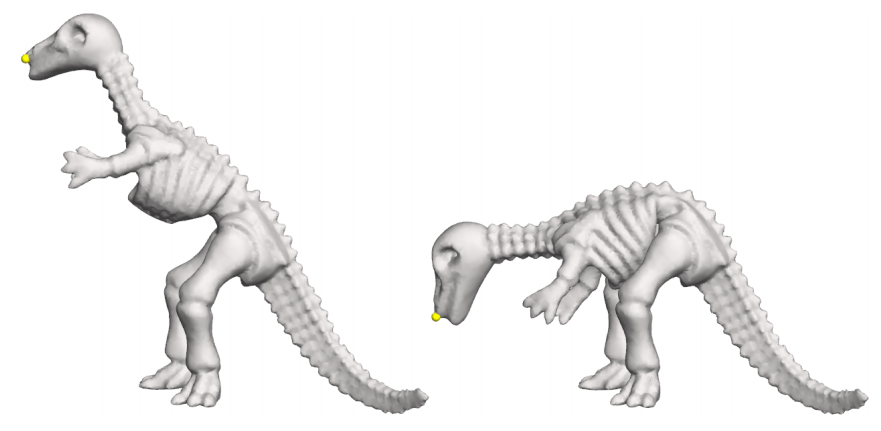
\includegraphics[width=0.35\linewidth]{dino_arap}}
    \caption{Dinosaur mesh undergoing ARAP deformation, obtained by translating the highlighted yellow vertex. Reprinted from~\cite{sorkine2007rigid}.}
    \label{fig:arap_dino}
\end{figure}      

Once aligned, a $d$-dimensional \emph{shape space} can then be defined (with $d << n$), where each $w \in \R{d}$ gives rise to a vertex configuration in $\R{3}$ (with unchanged triangulation). In this way, every plausible 3D example has a parameter vector $w \in \R{d}$ that generates it. This construction can then be interpreted as a \emph{generative} model. However, very few selections of $w \in \R{d}$ will generate a plausible-looking 3D mesh. This can then be interpreted probabilistically, by defining a density function $f(w)$ that defines the likelihood that a realistic 3D example would be represented by $w$ in shape space. 

\subsection{Modelling shapes (e.g. faces)}

The concepts raised above were first introduced in the seminal work of Blanz and Vetter~\cite{blanz-vetter}. They define a linear generator function based on principle component analysis (PCA) in order to map $d$-dimensional parameter vectors to the set of $n$ vertex coordinates. In particular they use the mapping:

\begin{equation}
    c(w) = \hat{c} + Ew
\end{equation}

where $c: \R{d} -> \R{3n}$ is the generator function, $\hat{c} \in \R{3n}$ is the mean 3D face in the training dataset and $E \in \R{3n \times d}$ is a matrix containing the $d$ most dominant eigenvectors computed over shape residuals $\{c_i - \hat{c_i}$. 

This construction assumes 3D faces in this $d$-dimensional parameter space follow a multivariate normal distribution (a concept explored further in this thesis Chapter 4). In addition, the function $f(w)$ which defines the likelihood shape space vector $w$ represents a plausible face, is therefore given by the Mahalanbois distance of $w$ to the origin. 

Note that this formulation additionally enables the definition of facial expressions. For example, Blanz and Vetter defined an expression (e.g. surprise) according to the difference in shape space between a expressive and neural face of the same subject. This then enabled the formulation above to be factored into identity and expression components:

\begin{equation}
    c(w_{idt}, w_{exp}) = \hat{c} + E_{idt}w_{idt} + E_{exp}w_{exp}
\end{equation}

where $E_{idt}, E_{exp}$ are the basis vectors of the identity and expression space and $w_{idt}, w_{exp}$ are the coefficients. As noted by Lewis et al.~\cite{xxx}, the basis vectors of the expression space above can be interpreted as a data-driven \emph{blendshape model}: a standard approach in the animation industry for representing facial expressions as a linear combination of target faces. This concept will later reemerge in a section discussing corrective blendshapes uses in SMPL~\cite{loper15smpl}.

%Blendshape Facial Animation
As identified by Blanz and Vetter, improved modelling of finer details (particularly around the eye or nose regions) can be obtained through local modelling. Various authors~\cite{xxx} began manually segmentating the face into parts and learning individual PCA representations for them. Later, segmentations were automatic and learned based on displacement patterns found in the training dataset. Next, approaches were adopted based on hierarchical, multi-scale frameworks~\cite{xxx, xxx}. Possibly the closest to later sections which require a focus on \emph{pose deformation}  is the work of Wu et al~\cite{xxx}. who combine a a local shape space model with an anatomical bone structure that helps regularize deformation. 

% booth et al 2017
% pascal 2010
% egger et al 2016b
% zhou et al.
% xu et al (deep 3d portrait from a single image)

A standard challenge in face modelling is towards reconstructing appearance, typically incorporating albedo and illumination (although frequently these are not factored, in which case apperance is generally referred to as \emph{texture}). Early work modelled shape and texture independently~\cite{xxx, xxx}, although recent techniques show solving for these factors jointly enable constraints to be applied due to correlations present. Perhaps most interesting are the recent techniques among these~\cite{xxx, xxx}, who propose methods based on deep convolutional models to jointly model shape and texture.  

% PROBLEMS
% the statistics of most models are limited to the face and do not include information on eyes, mouth interior or hair
% Second, the interpretability of the representations would benefit from being improved. PCA is the most commonly used method to perform statistics on 3D faces, and as it is an unsupervised method, the principal components do not coincide with attributes that humans would use to describe a face


\subsection{Modelling articulation (e.g. hands)}


% Perhaps the biggest difference with hand modelling are the complex modes of articulation among subjects. 


3D morphable models have also influenced work in 3D hand tracking and modelling. Human hands servce multiple purposes in everyday life, serving a mechanism to handle tools/objects, expressing emotion and aiding (or even as the primary tool for) communication. As a result, hands (and particularly fingers) exhibit complex articulation patterns which are best characterized as 3D \emph{rotations}. Compared to the previous section, in which face shape variation could be represented as as an abstract linear basis learnt from scans, an advantage to modelling hands is the modes of articulation can be defined in advance. 

In particular, human hand motion is controlled by a hierarchical bone structure referred to as a \emph{skeleton}. The point at which two bones meet is referred to as a \emph{joint} and can be used to define acceptable centers of articulation. The direction and magnitude of the articulation can then be neatly expressed as a 3D rotation.

This formulation helps provide insight into why the abstract linear basis (shape space) introduced in the previous section would be poor choice for modelling hands. Deformation is here characterized in terms of 3D rotations, and 3D rotations are non-linear with respect to the input angle. This is easily shown: 

\subsubsection{Primer on 3D rotations}

The simplest kind of 3D rotation is an \emph{elementary rotation} and involves a rotation around a single axis of a coordinate system. For example, the following matrix represents a rotation by an angle $\gamma$ around the $x$ axis:

\begin{equation}
    R_{x}(\gamma) = \begin{bmatrix}
        1 & 0 & 0 \\
        0 & \cos(\gamma) & -\sin(\gamma) \\
        0 & \sin(\gamma) & \cos(\gamma)
    \end{bmatrix}
\end{equation}

One can then apply this matrix to an input point $p \in \R{3}$ to compute the new position $p'$ after rotating $\gamma$ around the $x$ axis:

\begin{equation}
    p' = R_{x}(\theta)p
\end{equation}

This formulation can then be extended to represent any 3D rotation as the composition of elementary rotations. For example, a 3D rotation can be decomposed into a $\gamma$ rotation around the $x$-axis (pitch), followed by a $\beta$ rotation around the $y$-axis (yaw) and finally by an $\alpha$ rotation around the $z$-axis (roll). 

\begin{equation}  
    R = R_{z}(\alpha) R_{y}(\beta) R_{x}(\gamma)
\end{equation}

One can see immediately that affecting a 3D rotation (i.e. computing the new position of the points) is a non-linear function of the input angle. It is necessary, therefore to describe an alternative technique for low-dimensional and efficient mesh deformation, which relies on \emph{rigging} and \emph{linear blend skinning}. 

% Compared to facesCompared to faces, hands have a simpler space of shape variation (typically restricted to palm size, finger lengths etc.) but the modes of articulation are extremely complex. In the class of 3DMMs, hand models arguably have the strongest synergy to their biological counterparts; in many cases each of the 27 hand bones (occasionally except the capal bones which join the fingers to the wrists) are explicitly represented in the model skeleton.

\subsubsection{Skeletal Rigging and Linear Blend Skinning}

In cases that the articulated object is known in advance, it is common to augment a representative 3D mesh model with an internal skeleton that approximates the biological counterpart. This is achieved through a process known as \emph{rigging}.  

% In general, the mesh skeleton approximates the real, biometric skeleton by allowing the important modes of deformation but often is a rough approximation of the real, biometric skeleton be detailed enough to allow the primary modes of deformation, but often it is not necessary that the 3D mesh skeletthat the articulated object is known In cases that the mesh shape is known in advance, it is common to follow a process known as \textit{rigging}, in which the mesh is augmented with a hierarchical bone structure. The point at which two bones meet is called a \emph{joint}, and these can be used to define acceptable centres of rotation for mesh deformation. It is possible to describe a distribution of joint configurations, which could be used to constrain the mesh to (in the case of human / animal subjects) anatomically achievable poses. It is also simple to define conceptual `body parts' from a rigged mesh, by considering regions between pairs of joints; for example a lower leg region can be defined between a knee and ankle joint. A simple example of a rigged 2D mesh with joints indicated by green diamonds is shown in Figure~\ref{fig:finger_model}. Note how the mesh surface deforms naturally as the joints are displaced.

% \begin{figure}[H]
%     \centering
%     \begin{subfigure}{0.48\linewidth}
%     \centering
%         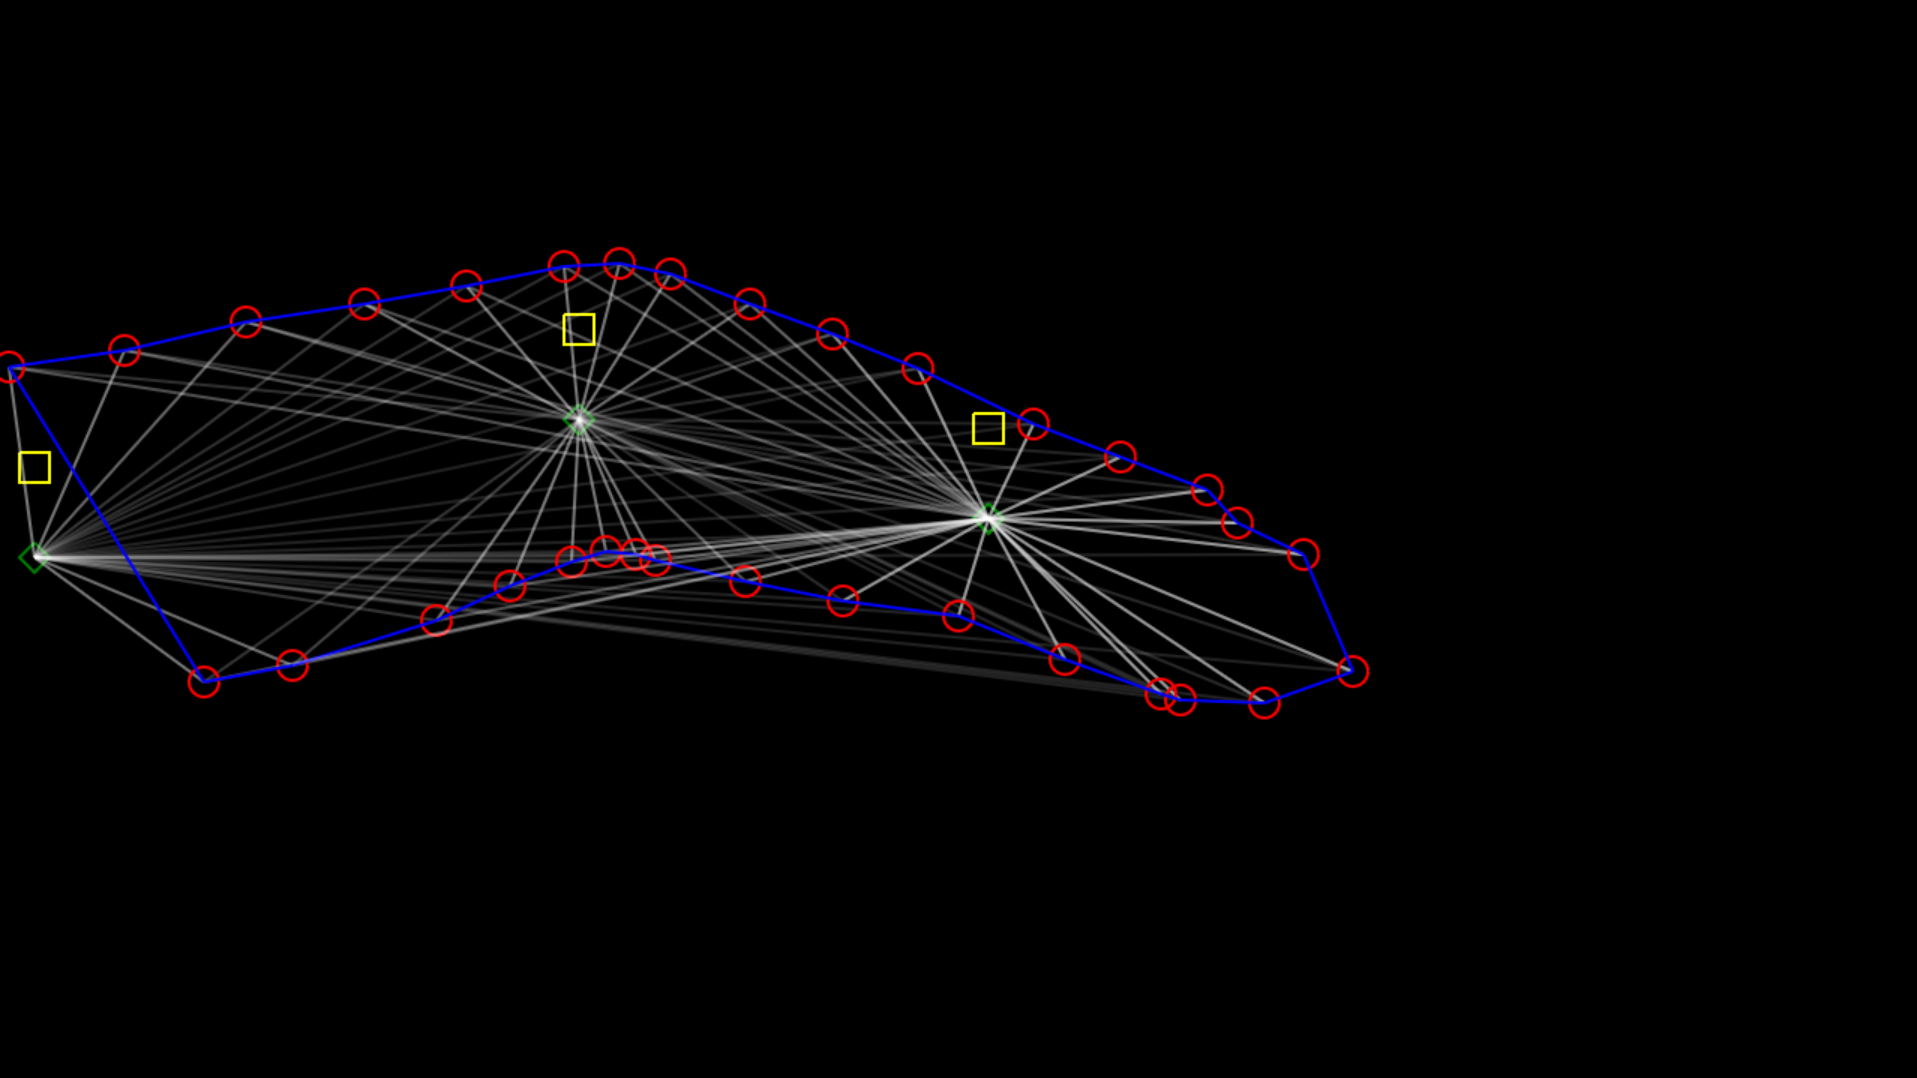
\includegraphics[width=1\linewidth]{finger/finger1}
%         \caption{Default joint positions.}
%     \end{subfigure}
%     \begin{subfigure}{0.48\linewidth}
%     \centering
%         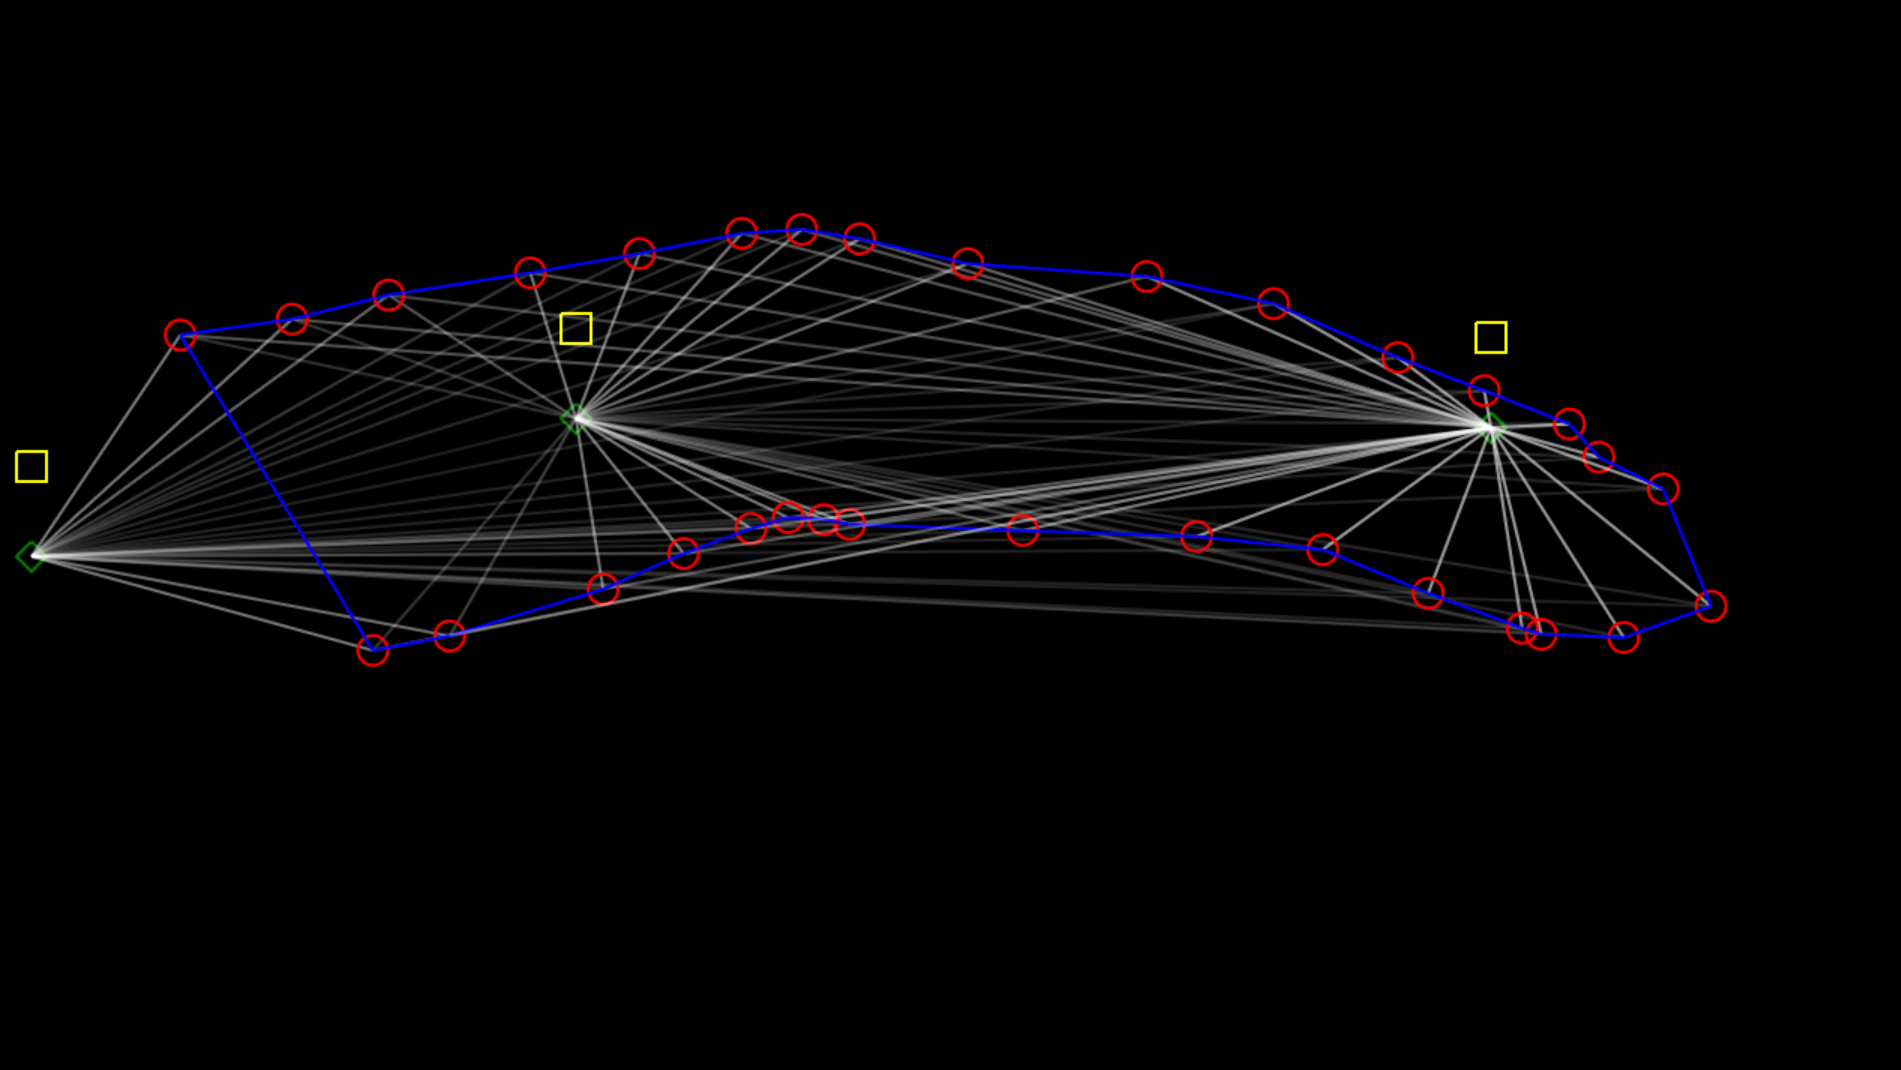
\includegraphics[width=1\linewidth]{finger/finger2}
%         \caption{Right-most joint displaced.}
%     \end{subfigure}
%     \begin{subfigure}{0.48\linewidth}
%     \centering
%         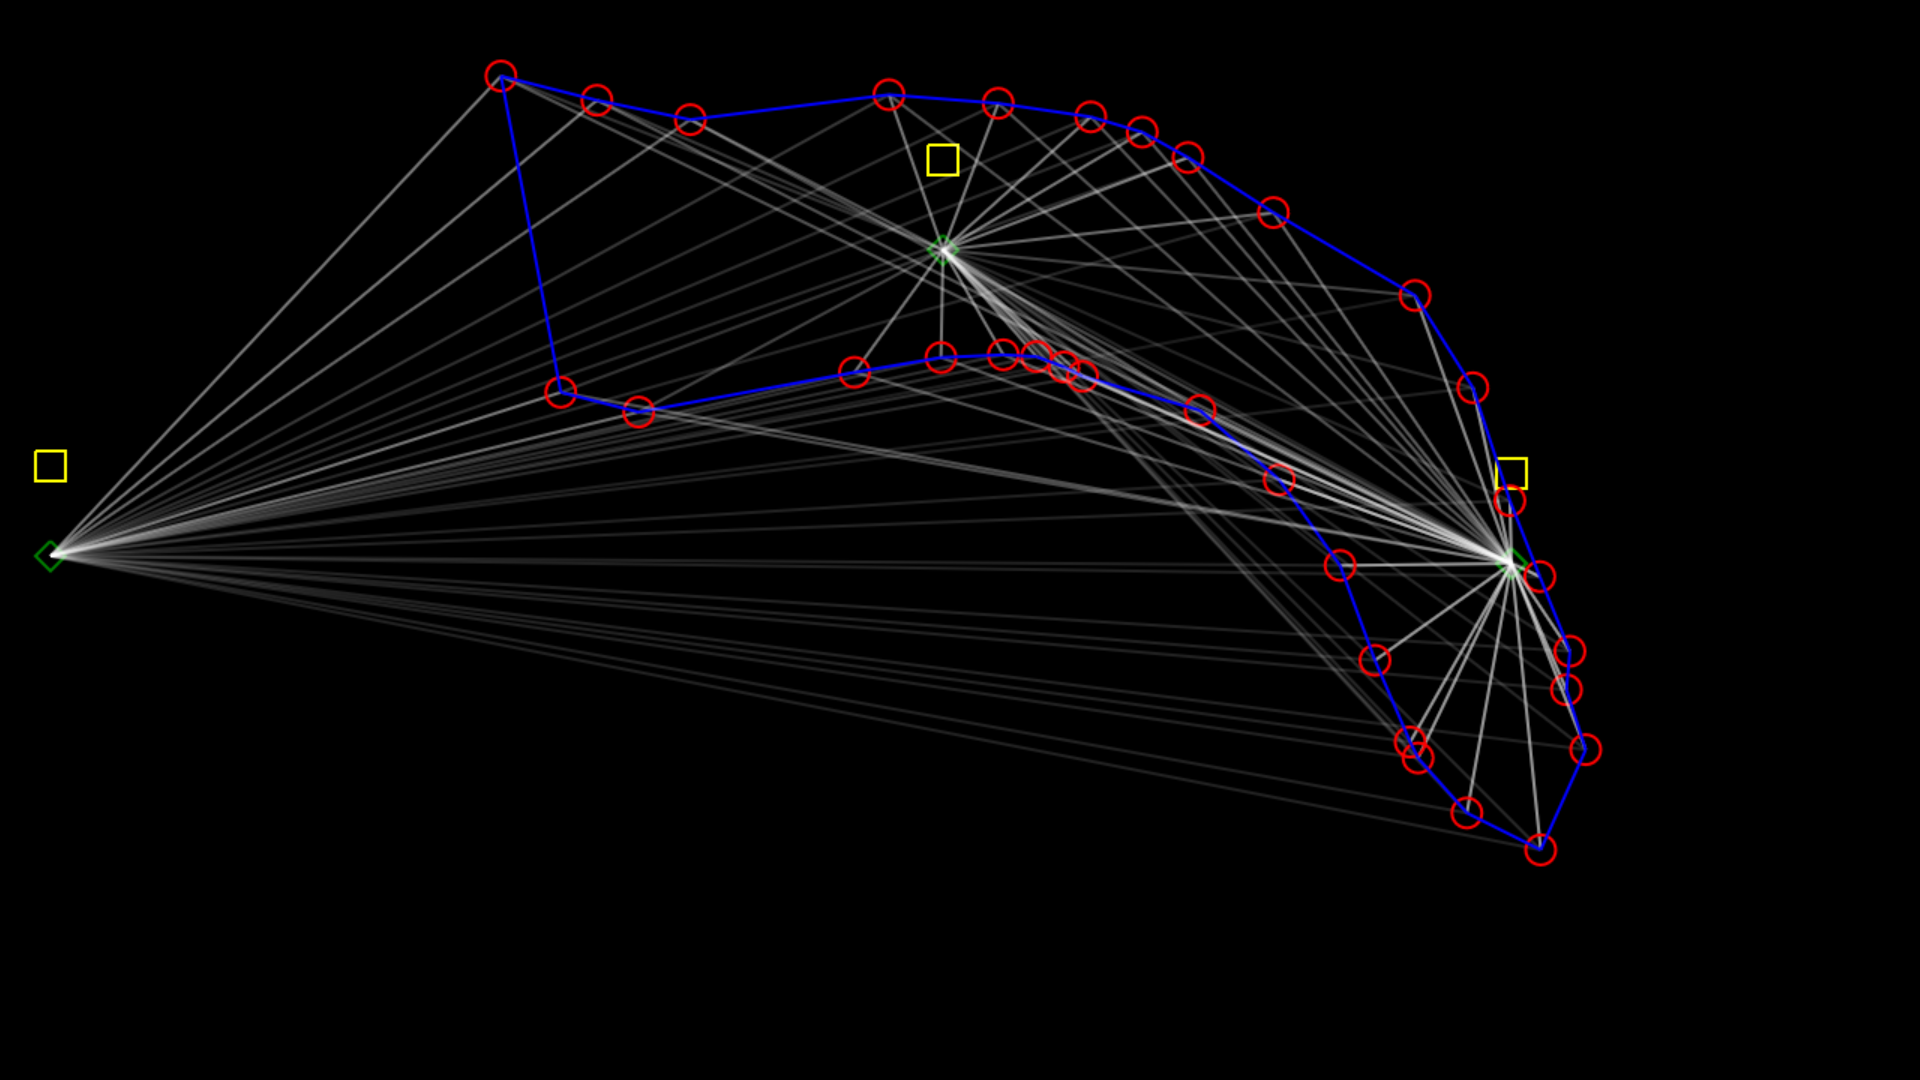
\includegraphics[width=1\linewidth]{finger/finger3}
%         \caption{Central joint displaced and right-most joint displaced and rotated.}
%     \end{subfigure}%
%     \caption{Web application demonstrating LBS on a 2D finger mesh. Joints are denoted as green diamonds.}
%     \label{fig:finger_model}
% \end{figure}

Formally, a skinned mesh consists of a set of rigged vertices $V \subseteq \R{3} \times \R{|J|}$, a set of faces $F \subseteq V^3$ and joint transformation matrices $J \subseteq \RR{3}{4}$. Each vertex $v = (x, s) \in V$ consists of positional coordinate $x \in \R{3}$ and a weight vector $s \in \R{|J|}$ which describes the level of influence each joint $j \in J$ has over its movement. Many approaches exist for assigning weights, but perhaps the simplest is to build a vector with entries corresponding to the distance from the vertex to each joint centre. Skinning weight vectors are normalized such that their entries sum to one, and for computational reasons, the number of non-zero elements is typically limited to 2 or 4. The weakness of such models is that artifacts and other unrealistic deformations can occur around the model joints, particularly for meshes that model non-linear structures such as humans. However, the technique is frequently used in computer graphics and game design when a character's shape is known ahead of time.

% To assist in explanation, Figure \ref{fig:rigged_cylinder} shows skinning weight influences from three joints within a rigged cylinder mesh. Here, $|J| = 3$ and each vertex $v_{i} = (x_{i}, s_{i}) \in V$ has a skinning weight vector $s_{i} \in \mathbb{R}^{3}$. Each model joint is assigned a distinct RGB value, shown separately in (a), (b) and (c), and together in (d) by linearly combining the colours. This linear blend colorization scheme will be frequently used in later sections of this report.

% \begin{figure}[H]
%     \centering
%     \begin{subfigure}{0.25\linewidth}
%     \centering
%         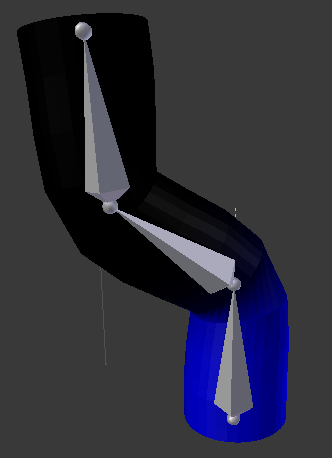
\includegraphics[width=1\linewidth]{wonky_pole/lower_bone}
%         \caption{Lower joint.}
%     \end{subfigure}%
%     \begin{subfigure}{0.25\linewidth}
%     \centering
%         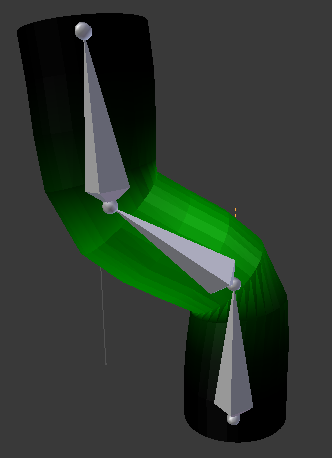
\includegraphics[width=1\linewidth]{wonky_pole/middle_bone}
%         \caption{Middle joint.}
%     \end{subfigure}%
%     \begin{subfigure}{0.25\linewidth}
%     \centering
%         
\includegraphics[width=1\linewidth]{wonky_pole/upper_bone}
%         \caption{Upper joint.}
%     \end{subfigure}%
%     \begin{subfigure}{0.25\linewidth}
%     \centering
%         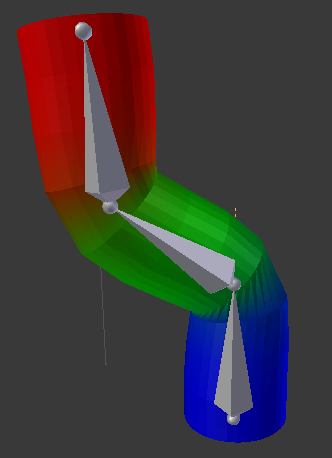
\includegraphics[width=1\linewidth]{wonky_pole/linear_blend}
%         \caption{Linear blend.}
%     \end{subfigure}%
%     \caption{A rigged cylinder with $|J| = 3$ and where each vertex $v_{i} = (x_{i}, s_{i}) \in V$ has a skinning weight vector $s_{i} \in \mathbb{R}^{3}$.}
%     \label{fig:rigged_cylinder}
% \end{figure}

% Figure \ref{fig:rigged_quadruped} shows a more complex rigged quadruped mesh with $|J| = 25$ with skinning weight influences again shown by the linear blend colorization scheme. Again, each joint is assigned a unique RGB value and a vertex's colour is calculated by linearly combining joint colours with skinning weight vectors given by the $\{s_{i}\}$. A triangle's colour is then generated by averaging the colours given for the three surrounding vertices.

% \begin{figure}[H] % Example image
%     \center{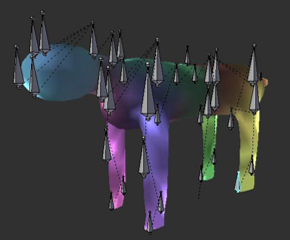
\includegraphics[width=0.5\linewidth]{linear_blend_bold_bones}}
%     \caption{A rigged quadruped with $|J| = 25$ and where each vertex $v_{i} = (x_{i}, s_{i}) \in V$ has a skinning weight vector $s_{i} \in \mathbb{R}^{3}$. Visualization uses the linear blend colorization scheme in which each joint is assigned a unique RGB value.}
%     \label{fig:rigged_quadruped}
% \end{figure}

Once a mesh has been suitably rigged, Linear Blend Skinning (LBS) can be used to apply the mesh deformation. Typically, a user assigns a transformation (e.g. rotation and translation) to each `joint' and LBS computes the an updated position of vertex $v = (x, s)$ where $x$ is the original location and $s = \{s_j\}$ are the skinning weight influence of joints $j$. The matrix $U_{j}$ (occasionally referred to as a the \emph{reference pose}) is the mapping from the bone's "default" coordinate system to world coordinates. As a result, it need only be computed (and inverted) once since it is invariant to changing joint angles. In general, a user will supply the matrices $D_{j}$ to define the mapping from the bone's deformed coordinate system to world coordinates.

The updated position of an input point $x$ can then be calculated by LBS:

\begin{equation}
    LBS(D, x; U, s) = \sum_{j}s_{j}D_{j}U_{j}^{-1}x
\end{equation}

% TODO: Explain LBS for kinematic trees
Note this formulation is made slightly more complicated in the case of kinematic trees, since the 

Similarly to the approach mentioned above, this formulation can again be seen as a generative 3D model. In particular, an output vertex positions $v'$ can be computed from a vector of 3D joint rotations $\theta$ and input vertex position $v$ as follows:

\begin{equation}
    v' = LBS(R(\theta), v)
\end{equation}

\subsubsection{3D Deformable Hand Modeling}

With the above formulation, it is now possible to give an overview of recent hand tracking literature. In many cases, 3D morphable hands models are built to reflect the 27 biological hand bones (occasionally except the capal bones which join the fingers to the wrists). Of course, while the major source of hand deformation is due to 3D pose, some sources of variation are present due to hand size and finger propotions.

Allen et al~\cite{xxx} handle this variation adapting a 3D surface with displacement maps with various constraints designed to avoid self-intersections before adopting the linear blend skinning formulation defined above. Rhee et al~\cite{xxx} learn a shape deformation space (with a similar technique to that of faces) and user-specific skinning weights for LBS. Albrecht undergo a laborious process to create extremely detailed hand models through laser scanninng plaster casts~\cite{xxx}. A significant advance was presented by Taylor et al~\cite{xxx}. who presented a method to learn a personalized hand model (although not a shape basis) given an input video sequence (with depth) taken of a user slowly articulating their fingers. Ballan et al.~\cite{xxx} follow a similar process by making use of multi-view input. 


% TODO: Allen et al. B. Allen, B. Curless, and Z. Popovic. Articulated body de-formation from range scan data. In ACM Transactions on Graphics (TOG). ACM, 2002. 2

% Represent the model as an adaptation of a standard subdivision surface model with linear blend skinning. Cruicially their adaptations are displacement maps on top of a base surface. The displacements must be limited in magnitude to avoid self-intersections and their shape basis is forced to coincide with the input scans.

% % TODO: Rhee et al. T. Rhee, U. Neumann, and J. P. Lewis. Human hand modeling from surface anatomy. In Proceedings of the 2006 symposium on Interactive 3D graphics and games, pages 27–34. ACM, 2006. 2

% Early work included the work of Rhee et al.~\cite{xxx} who learn a 3D shape deformation space from hands by fitting 3D model with user-specific skinning. 

% % TODO: Albrecht et al. I. Albrecht, J. Haber, and H.-P. Seidel. Construction and animation of anatomically based human hand models. In Proc. Eurographics, 2003. 2

% Albrecht et al. go to the other extreme creating very detailed, physically-realistic hand models. However, the process is laborious requiring plaster casting of human hands, performing laser scans, and manually creating a physics-enabled hand model.

% % TODO: Taylor et al. J. Taylor, R. Stebbing, V. Ramakrishna, C. Keskin, J. Shotton, S. Izadi, A. Hertzmann, and A. Fitzgibbon. User-specific hand modeling from monocular depth sequences. In Proc.CVPR, 2014. 1, 2, 4, 5, 7

% A more automatic technique is presented by Taylor et al., which generates personalized hand models given noisy input depth sequences where the user’s hand rotates 180 degrees whilst articulating fingers. A continuous optimization that jointly solves for correspondences and model parameters across a smooth subdivision surface with as rigid as possible (ARAP) regularization leads to high-quality userspecific rigged hand models, though not a shape basis. Whilst the process is automatic, the hands are required to cover the full range of articulations, and longer sequences are required, leading to more complex capture requirements and more costly optimization.

% % TODO: Ballan et al. L. Ballan, A. Taneja, J. Gall, L. V. Gool, and M. Pollefeys. Motion capture of hands in action using discriminative salient points. In Proc. ECCV, 2012. 1, 2

% Ballan et al. construct a personalized hand
% mesh using a multiview camera rig and Poisson surface reconstruction, which is then manually skinned. They demonstrate high-quality results with complex two-handed and
% hand-object interactions, closely fitting the detailed mesh
% model to the data. However, this system focuses on pose
% estimation as opposed to the shape construction, which is
% performed in an time consuming manual manner.

% TODO: Khamis et al. Learning an efficient model of hand shape variation from depth images

% TODO: Fits Like a Glove: Tan et al. https://www.microsoft.com/en-us/research/wp-content/uploads/2016/06/FitsLikeAGlove.pdf



% TODO: Taylor et al. Efficient and Precise Interactive Hand Tracking Through Joint, Continuous Optimization of Pose and Correspondences

\subsection{Modelling the human body surface}

% hasler et al. 2010

However, of all human categories, the works of most relevance to this thesis are those which represent the entire human body surface. It is first important to characterize these two deformation modes which must be overcome with modelling algorithms. Firstly, there is considerable variation in the \emph{shape} characteristics between different human subjects. Humans not only vary in their heights and weights, but also in their body part proportions, muscle density, fat etc. Secondly, humans exhibit significant \emph{pose} variation, characterized by the range of motion of body parts (e.g. arms and legs). In general, pose is likely to change for a individual subject over a sequence. 

The earliest deformable 3D models of the human body was presented by Allen at al~\cite{xxx} (although ~\cite{xxx} came soon after with similar ideas). Allen et al. learnt a PCA shape space model from 250 registered body scans cound in the CAESAR dataset. The model was articulated through a set of pose parameters, which use linear blend skinning to interpolate rotation matrices assigned to the joint to transform model veertices. Unfortunately, this approach suffers from artefacts around joint locations, due to a loss of volume. For this reason, it is important to note that pose and shape are not entirely independent; in fact, body shape does indeed change due to pose variation. Imagine for example, how a fatty stomach region would deform during a walking sequence. SCAPE~\cite{anguelov05scape} improved over this by introducing a model equipped with both body shape variation and pose-dependent shape changes, expressed in terms of triangle deformations (rather than vertex displacements, see~\cite{loper15smpl} for a comprehensive overview). An important advance was made by Hasler et al.~\cite{xxx}, who learn two linear blend rigs: one for pose and one for body shape. In this model, shape change was controlled through the introduction of abstract bones that further deform the vertices.

Perhaps the most significant advance however, was the introduction of the Skinned Multi-Person Linear (SMPL) model of Loper et al.~\cite{loper15smpl}. SMPL follows a similar design philosophy to SCAPE by decomposing shape into identity-dependent and pose-dependent components. However, unlike scape, SMPL adopts a vertex-based skinning approach based on corrective blend shapes. The model's shape space is first taught how human beings deform through pose changes using 1786 high-resolution 3D scans of different subjects in a wide variety of poses. Following alignment to a template mesh, a linear model for each biological gender is created from the CAESAR dataset \cite{robinette2002civilian} using principal component analysis (PCA). SMPL can then be viewed as a function, which makes use of a shape basis and linear blend skinning to map a set of pose and shape parameters to a set of vertex locations. Precisely, \emph{pose} is given as a set of 3D rotations (per-joint and global) in axis-angle form $\pose \in \R{24}{3}$. \emph{Shape} is then given as coefficients for a learned shape basis $\shape \in \R{10}$. The SMPL function can then be viewed as:

\begin{equation}
    v = \SMPL(\pose, \shape) + \trans
\end{equation}

where $v \in \RR{6890}{3}$ and $\trans \in \R{3}$ is a global translation parameter. Further details on SMPL have been left to Chapter 5 of this thesis, which makes use of the model to examine uncertainty when deriving 3D reconstructions of ambiguous input imagery.

% Another key ambition for the SMPL model was the motivatio to create a realistic data-driven human body model which can be rendered in real-time using standard engines, such as Unity~\cite{unity2017} or Blender~\cite{blender2017}. Having been designed for animation, SMPLs base template has a number of useful qualities for this work; the underlying mesh is a clean structure and comprises relatively few polygons. A novelty of this model is that it encodes explicit and meaningful body joint positions. Some sample SMPL meshes are shown in Figure \ref{fig:smpl_model}.

% TODO: GHUML & GHUM model
More recently, SMPL has been combined with face and hand models to add expressive capabilities~\cite{xiang19monocular, joo18total, pavlakos19expressive}. CAPE~\cite{CAPE:CVPR:20} also shows how to add a clothing parameter to effectively model humans in clothing, a challenge solved by learning a shape prior over freeform vertex deformations Techniques have also been developed to model human clothing -- a common challenge generally handled by allowing SMPL model vertices to vary independently to the provided blend shapes. SMPL has also been recently improved with STAR~\cite{STAR:2020} which constructs a part-based shape space (closely related to the local PCA space discussed in the earlier shape section of this literature review). They show this new parameterization is much more efficient (uses approximately 20\% of the model parameters of SMPL) and avoids capturing spurious long-range correlations present in the training dataset. They also show a method for learning shape-dependent pose-corrective blendshapes, that better model how individuals with different body shapes deform with motion. Tangential work of Xu et al.~\cite{ghum-ghuml} train an end-to-end network and learn 3D human body model parameters (including faces and hands) for an input artist model using variational auto-encoders and normalizing flows. This work will be further explored Chapter 5 in which these generative models will be fully examined. 

\begin{figure}[H] % Example image
    \center{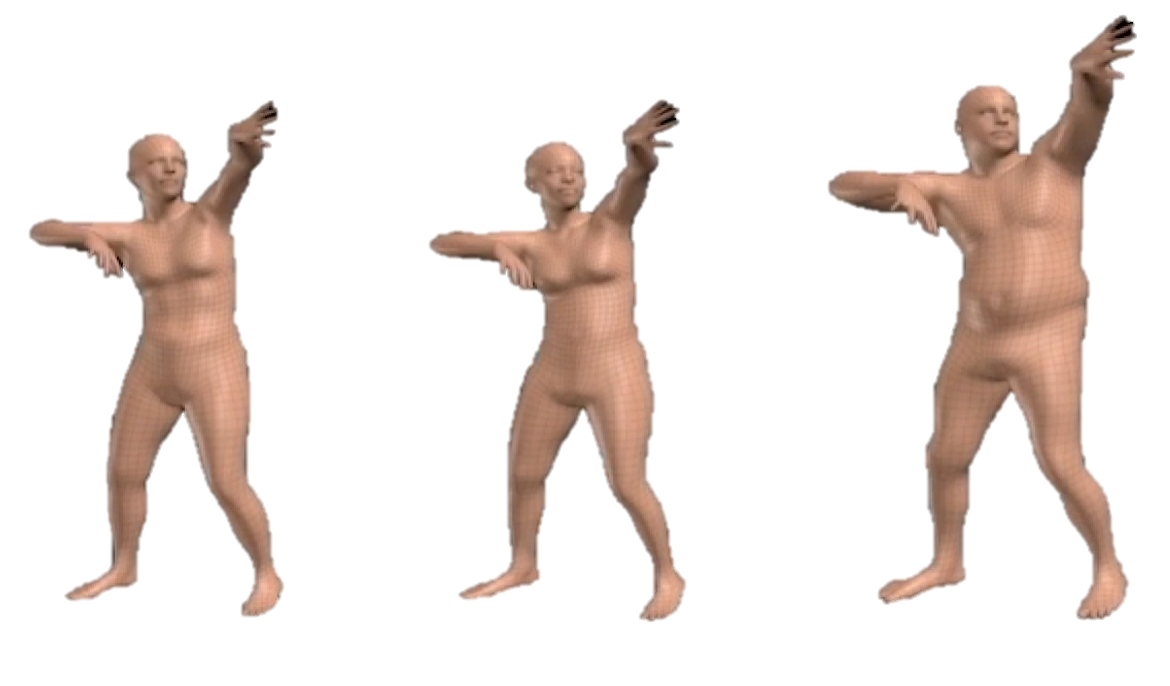
\includegraphics[width=0.5\linewidth]{smpl_wbg}}
    \caption{SMPL model showing pose-invariant shape changes, reprinted from~\cite{loper15smpl}.}
    \label{fig:smpl_model}
\end{figure}

\subsection{Modelling animals}

There is still relevatively little work specifically focusing on the 3D scanning~\cite{xxx} and modelling of animal categories. The variation in animal shape and sizes combined with the practical challenges associated with scanning live animal subjects (particularly in attaching traditional motion capture equipment) make scanning a difficult task. As a result, there is a significant lack of real 3D animal training data available in the public domain which could otherwise have been employed to build 3D deformable models. As with humans, animals deformations can again be factored into shape (e.g. variation mostly due to identity) and pose (variation due to articulated motion). However, the enormous diversity among animal species and even between individual breeds results in a much more complex shape space.

Some early work by Favreau et al~\cite{xxx} describe a method for animating an artist-designed rigged 3D model, by tracking a 2D sequence. Chen et al.~\cite{xxx} learn a shape space by registering 11 3D shark models downloaded from the Internet. Cashman et al.~\cite{xxx} learn a morphable model of dolphin shapes by adapting a representative 3D model to 2D images. Ntouskos et al.~\cite{xxx} fit geometric primitives to manually-segemented animal parts generated from an input collection. Reinert et al.~\cite{xxx} demonstrates an effective method for fitting generalized cylinders to an input video sequence supplied with sketched limb tracks. They demonstrate reconstructed results with 3D texture on a few quadruped sequences. So far, none of these techniques for animal reconstruction explicitly factor shape and pose.

\subsubsection{SMAL}
A similar technique to that used to build the SMPL model has been recently used to build a Skinned Multi-Animal Linear Model (SMAL)~\cite{zuffi2017menagerie}, a generative animal model exhibiting realistic 3D shape (see Figure \ref{fig:smal_model_shape}) and pose (see Figure \ref{fig:smal_model_poses}). Due to the lack of available motion capture data for animal subjects, the SMAL model is learnt from a set of $41$ 3D scans of toy figurines in arbitrary poses. The figurines span five quadruped families, and included examples of lions, cats, tigers, dogs, horses, any many more, although notably for this work no rodent toys were included. The paper introduces a new technique to accurately align each toy scan to a common template, allowing the shape space to be learnt.

\begin{figure}[H]
    \centering
    \begin{subfigure}{0.3\linewidth}
    \centering
        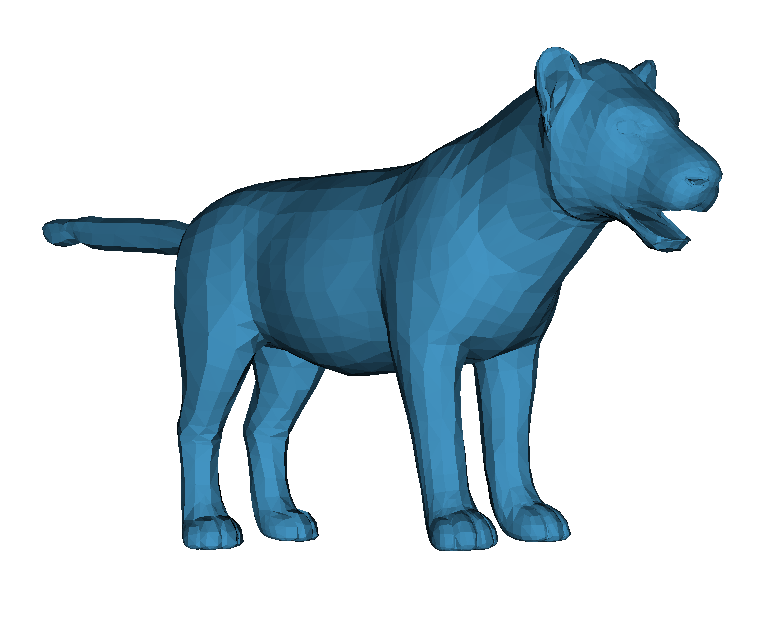
\includegraphics[width=1\linewidth]{smal/default}
        \caption{Default SMAL mesh.}
    \end{subfigure}%
    \begin{subfigure}{0.3\linewidth}
    \centering
        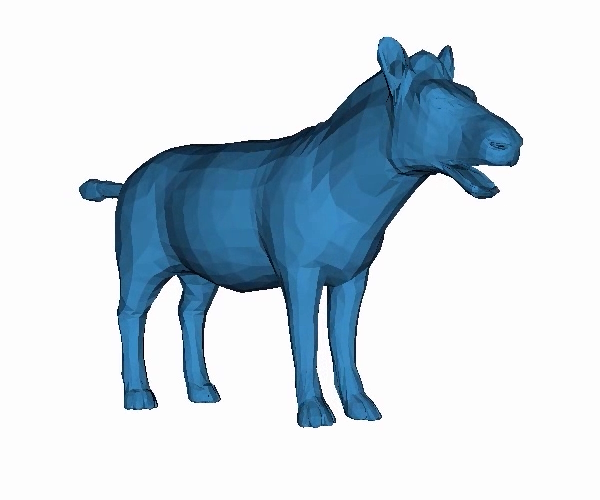
\includegraphics[width=1\linewidth]{smal/horse}
        \caption{SMAL in horse shape.}
    \end{subfigure}%
    \begin{subfigure}{0.3\linewidth}
        \centering
            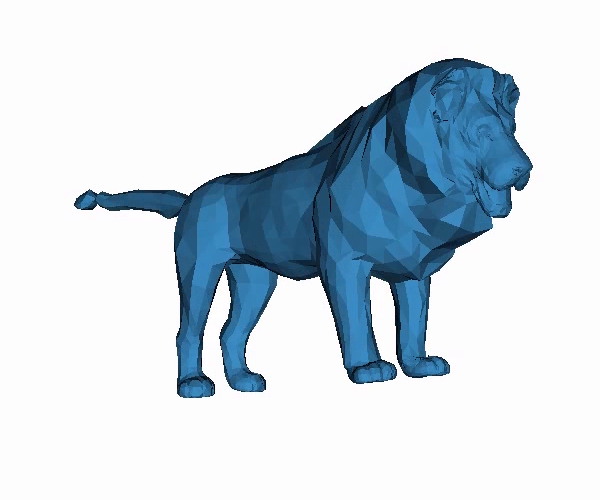
\includegraphics[width=1\linewidth]{smal/lion}
            \caption{SMAL in lion shape.}
    \end{subfigure}%
    \caption{SMAL with varying shape parameters.}
    \label{fig:smal_model_shape}
    \end{figure}

    \begin{figure}[H]
    \centering
    \begin{subfigure}{0.3\linewidth}
    \centering
        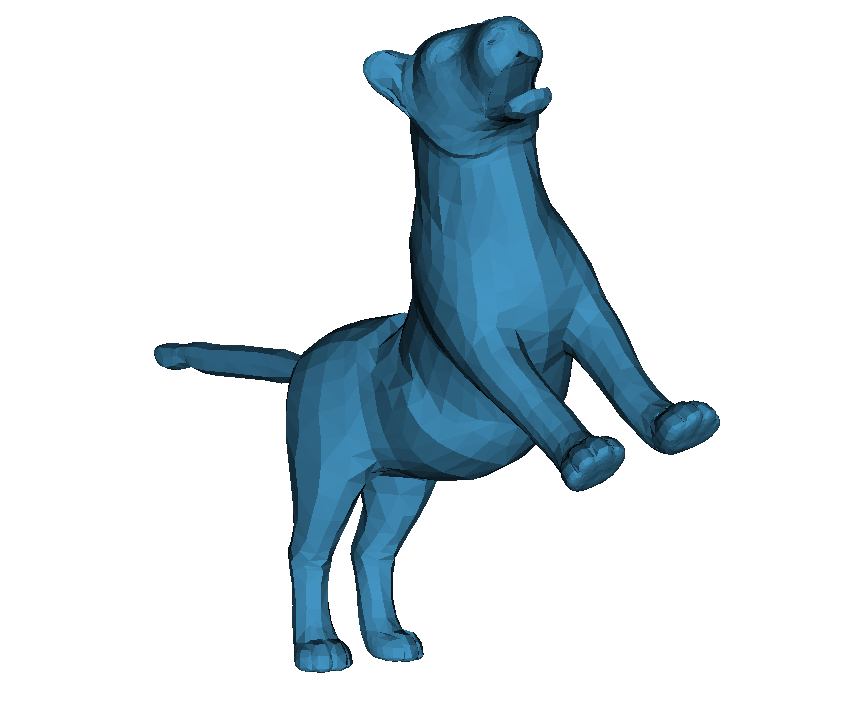
\includegraphics[width=1\linewidth]{smal/pose_1}
    \end{subfigure}%
    \begin{subfigure}{0.3\linewidth}
    \centering
        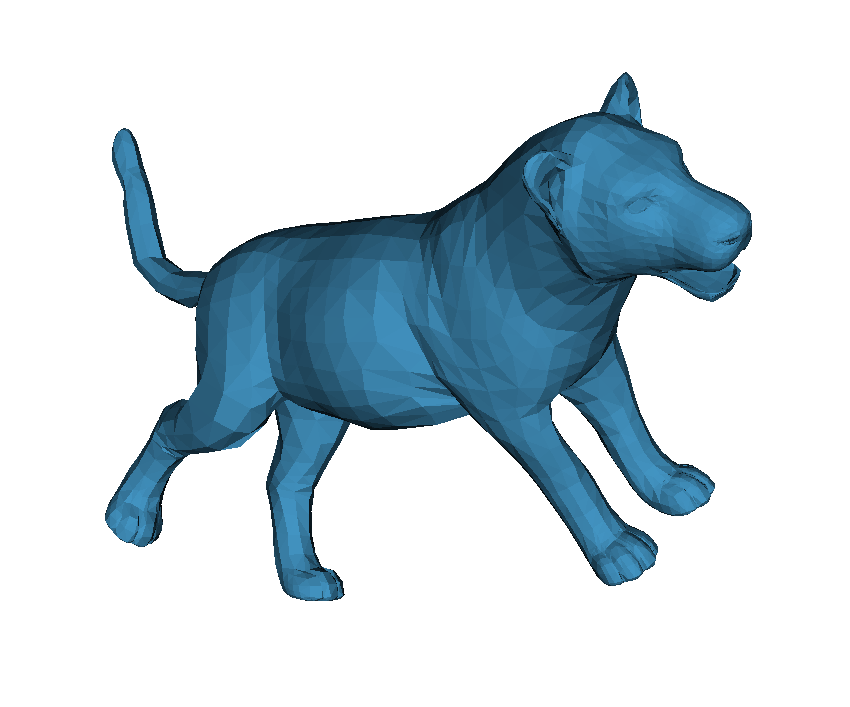
\includegraphics[width=1\linewidth]{smal/pose_2}
    \end{subfigure}%
    \begin{subfigure}{0.3\linewidth}
        \centering
            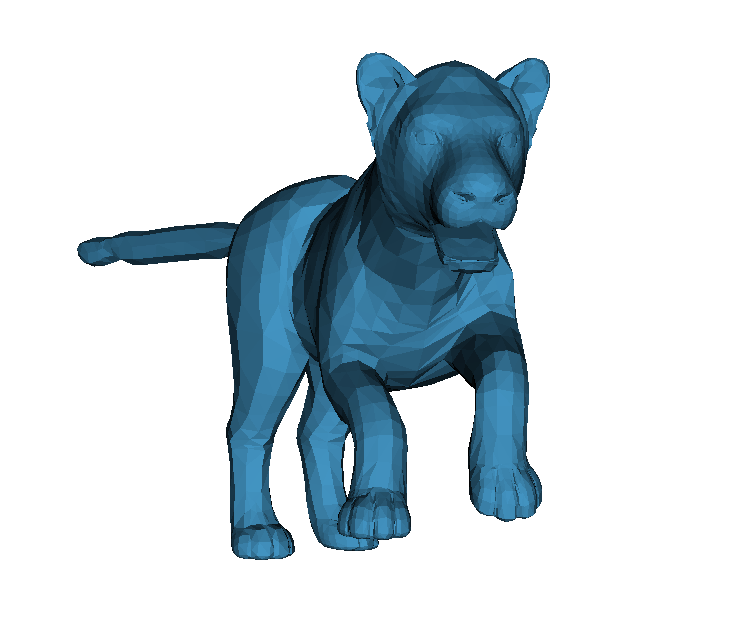
\includegraphics[width=1\linewidth]{smal/pose_3}
    \end{subfigure}%
    \caption{SMAL with varying pose parameters.}
    \label{fig:smal_model_poses}
\end{figure}

From the paper, SMAL is defined as a function $\SMAL(\pose, \shape)$ parameterized by pose-invariant shape $\shape \in \R{41}$ (again, coefficients of a low-dimensional shape space) and pose $\pose \in \RR{32}{3}$ (including global rotation). There are three pose parameters for each of the $32$ body joints and an additional three to express the global rotation. Global translation $\gamma$ is expressed by a further three parameters. The $\SMAL$ function returns a triangulated surface comprising $6890 \times 3$ vertex locations. Chapters 3 and 4 of this thesis make use of the SMAL model in order to reconstruct various quadruped categories.

\section{Methods for monocular reconstruction of articulated subjects}

    Having discussed methods for modelling articulated subjects, this section will discuss approaches for reconstructing the 3D shape and pose of a subject from a monocular image or video. It is important to note that this task is challenging and fundamentally ill-posed. In common with other challenging 3D reconstruction tasks, input images will typically exhibit variation in camera view, lighting and environmental occlusion. However, 3D reconstruction pipelines for articulated subjects must also deal with variation due to body shape, body pose, clothing and self-occlusion (body parts obscuring other parts). In addition, the challenge of reconstructing 3D models from 2D images is also inherently ambiguous. As explained by Toshev and Szegedy~\cite{toshev2014deeppose}, even if 2D structure can be determined (for example, using 2D keypoint prediction), the subsequent `lifting' step to recover 3D remains ill-posed, as the space of consistent 3D poses for given 2D landmark locations is infinite. It is for this reason that the history of monocular 3D reconstruction makes extensive use of 3D morphable models (or other geometric, temporal, structural priors), as they provide necessary optimization contraints.

    The theme of this section is therefore to discuss how 3D morphable models (3DMMs) can be incoporated into 3D reconstruction pipelines. In general, algorithms take as input an image or video and predict a set of 3D model parameters $\alpha$ (often factored into shape $\shape$ and pose $\pose$). Once determined, the output parameters are then supplied to the morphable model's generator function $g: \alpha \mapsto \R{3}$ (e.g. $\SMPL: (\shape, \pose) \mapsto \R{3}$ or $\SMAL: (\shape, \pose) \mapsto \R{3}$) to produce vertex positions $V \subseteq \R{3}$ for the model $M = (V, T)$ with fixed triangulation $T$. For completeness and comparison, this section will make some mention of the small class of 3D reconstruction methods for articulated subjets which operate without an explicit 3D morphable model. Although currently a developing area, current work in this category typically requires either paired 3D training data, employ alternative (and arguably more restrictive) shape priors (e.g. symmetry constraints) or produce results of significantly lower fidelity.

    Methods which align a parametric 3D model to monocular input date back as far as 1963, in a seminal paper by Roberts~\cite{xxx}. Roberts presents a method which optimizes parameters for viewpoint and cuboidal shape primitives to reconstruct a 2D line image. Model-based methods have also been applied to understand object structure, starting with fitting of geometric primitives~\cite{xxx} and later with Active Shape Models~\cite{xxx} which learn deformation priors from a provided training set. Perhaps due to the numerous commercial applications, the majority of recent work in 3D shape and pose recovery focuses particuarly on \emph{humans} as a special case. The first example of such an approach is the seminal work of Blanz and Vetter~\cite{blanz-vetter} who built the first 3D morphable face model by aligning 3D scans and optimized the parameters to provide a fit to a single image. Since then, the research community has collected a multitude of open source human datasets which provide strong supervisory signals for training deep neural networks. These include include accurate 3D deformable template models~\cite{loper15smpl} generated from real human scans, 3D motion capture datasets~\cite{ionescu2013human3,vonmarcard2018recovering} and large 2D datasets~\cite{lin2014microsoft,johnson2010clustered,andriluka14cvpr} which provide keypoint and silhouette annotations. The combination of these publically available datasets and their incoporation into deep learning pipelines have led to impressive reconstruction results when tested on in-the-wild human images and videos. Unfortunately, the diversity among animal subjects and the practical challenges associated with data capture have resulted in few datasets being made available. Despite appearing superficially similar to human tracking, these factors result in specific challenges to animal tracking which must be carefully handled. Perhaps for this reason, the body of related literature for animal tracking is considerably sparser. The remainder of this section will focus on methods for 3D pose estimation, followed by 3D shape and pose reconstruction of human and animal bodies. Further discussion on techniques for body part (e.g. face, hands) reconstruction are deferred to the following survey papers~\cite{xxx, xxx}.

\subsection{3D Pose Estimation}

% The reconstruction of an arbitrary configuration of 3D points from a single monocular RGB image has three characteristics that affect its performance: (i) it is a severely ill-posed problem because similar image projections can be derived from different 3D poses; (ii) it is an ill-conditioned problem since minor errors in the loca- tions of the 2D body joints can have large consequences in the 3D space; and (iii) it suffers from high dimensionality ( Agarwal and Triggs, 2006 ).

    Techniques for 3D pose estimation output a set of 3D keypoint locations which can be combined to form a skeletal outline. Apart from basic limb measurements, no other shape detail (e.g. surface definition, object density etc.) is obtained. However, it should be noted that this output form is often perfectly satisfactory depending on the intended application. In particular, this family of techniques have found numerous applications in controllerless gaming (e.g. Microsoft Kinect~\cite{kinectpaper}), motion capture (e.g. for digital character generation~\cite{xxx}), gait analysis (e.g. identifying lameness in cattle~\cite{xxx}) and many more. 
    
    The general approach is to recover a 3D skeleton such that the 3D joints project to known or estimated 2D joints subject to anatomical priors. Early approaches in this category fit human stick figures with various constraints, including assumptions of fixed limb lengths~\cite{xxx}, length ratios~\cite{xxx} or that limb lengths are isometric across individuals and vary only in global scaling~\cite{xxx}. More advanced techniques built statistical models of shape variation using anthropometric tables or learnt them from motion capture data~\cite{barron2001estimating}.

    A broad category of appraoches for this are methods for \emph{non-rigid structure from motion}~\cite{xxx}. The general formulation is to express a 3D skeleton $S \in \RR{3}{P}$ on $P$ points as a linear combination of basis shapes $S_{1}, \dots, S_{k}$ where $S_{i} \in \RR{3}{P}$. Precisely:
    
    \begin{equation}
        S = \sum_{i=1}^K l_{i} \cdot S_{i} \quad S, S_{i} \in \RR{3}{P} \quad l_{i} \in \R{}
    \end{equation}
    
    Assuming scaled orthographic projection, the following expression represents the projection of $P$ points of $S$ into 2D image coordinates $(u_{i}, v_{i})$:
    
    \begin{equation}
        \begin{bmatrix}
            u_{1} & u_{2} & \dots & u_{P} \\
            v_{1} & v_{2} & \dots & v_{P} \\
        \end{bmatrix}
        = R \cdot ( \sum_{i=1}^{K} l_{i} \cdot S_{i} ) + T
    \end{equation}

    or equivalently:

    \begin{equation}
        \begin{bmatrix}
            u_{1} & u_{2} & \dots & u_{P} \\
            v_{1} & v_{2} & \dots & v_{P} \\
        \end{bmatrix}
        = 
        \begin{bmatrix}
            l_{1}R & \dots & l_{K}R
        \end{bmatrix}
        \cdot
        \begin{bmatrix}
            S_{1} \\
            S_{2} \\
            \dots \\
            S_{K} \\
        \end{bmatrix}
    \end{equation}

    \def\PT#1#2#3{#1_{#2}^{(#3)}}
    \def\T#1#2{#1^{(#2)}}

    This can then be extended to handle multiple views of the subject taken over a monocular video sequence. Let $(\PT{u}{i}{t}, \PT{v}{i}{t})$ denote the tracked 2D point at timestep $t$. This gives rise to the following system, taken over $N$ timesteps:

    \begin{equation}
        \underbrace{
        \begin{bmatrix}
            \PT{u}{i}{1} & \dots & \PT{u}{P}{1} \\
            \PT{v}{i}{1} & \dots & \PT{v}{P}{1} \\
            \PT{u}{i}{2} & \dots & \PT{u}{P}{2} \\
            \PT{v}{i}{2} & \dots & \PT{v}{P}{2} \\
            & \dots & \\
            \PT{u}{i}{N} & \dots & \PT{u}{P}{N} \\
            \PT{v}{i}{N} & \dots & \PT{v}{P}{N} \\
        \end{bmatrix}
        }_{W}
        = 
        \underbrace{
        \begin{bmatrix}
            \PT{l}{1}{1}\T{R}{1} & \dots & \PT{l}{K}{1}\T{R}{1} \\
            \PT{l}{1}{2}\T{R}{2} & \dots & \PT{l}{K}{2}\T{R}{2} \\
            & \dots & \\
            \PT{l}{1}{N}\T{R}{N} & \dots & \PT{l}{K}{2}\T{R}{N} \\
        \end{bmatrix}
        }_{Q}
        \cdot
        \underbrace{
        \begin{bmatrix}
            S_{1} \\
            S_{2} \\
            \dots \\
            S_{K}
        \end{bmatrix}
        }_{B}
    \end{equation}

    % https://arxiv.org/pdf/1705.03098.pdf

    This shows the tracking matrix $W$ can be factored into 2 matrices: $Q$ which contains the camera pose $\T{R}{t}$ and configuration weights $\PT{l}{1}{t}, \dots, \PT{l}{K}{t}$ per frame ${t}$. $B$ encodes the $K$ basis shapes $S_{i}$. This system can be factored with singular value decomposition to yield the shape basis $S_{i}$, per-frame camera rotations $R$ and per-frame configuration weights $l$. A number of techniques follow this formulation~\cite{xxx, xxx, xxx}, but start with a shape basis learnt from available motion capture datasets (e.g. CMU~\cite{xxx}).

    More recent approaches were designed to be fully automatic. Shotton et al.~\cite{kinectpaper} designed a commerically-available system for 3D human skeletal tracking which required a depth sensor. A generative 3D body model was used to synthesize a large training dataset of depth images with corresponding body part labels. Density estimators for each body part are then used in combination to localize body joints with a calculated confidence value. Taylor et al.~\cite{taylor2012vitruvian} predict dense correpsondences between image pixels (again, with depth so in $\R{3}$) and a representative 3D human body model, again by training on synthetic depth images. Chapter 3 of this thesis demonstrates a technique for predicting keypoints by training on synthetic \emph{silhouette} data, rendered from an animal deformable body model, which overcomes the need for depth imagery at test time.

    Automatic monocular approaches often take advantage of 2D keypoint or body part detectors when reasoning about 3D skeletons. Simo-Serra et al.~\cite{xxx, xxx} form a probabilistic model that models both 3D pose and 2D keypoints jointly, overcoming noise among 2D body parts. Other approaches~\cite{xxx, xxx} employ a two-stage pipeline; they begin by localizing 2D joint positions on an input image before running a subsequent optimization step that `lifts` these to a 3D pose. Tangential work~\cite{xxx} takes uses detected 2D joints to perform a nearest neighbour search in a 3D mocap dataset. The most recent two-stage pipelines rely on deep convolutional networks to predict keypoints. Examples of such systems include DeepPose~\cite{toshev2014deeppose}, an approach which employs a CNN to reason jointly about 2D landmark detection and 3D pose estimation from single RGB images. Pishchulin et al.~\cite{pishchulin2016deepcut} later introduced DeepCut which extends DeepPose to the multi-person case.

    State-of-the-art techniques now operate as a direct regression to a 3D pose. Most often, paired 3D training data (such as is available from datasets such as Human3.6M~\cite{xxx}) is required which is generally expensive to obtain, particularly for animal categories. One branch of approaches~\cite{tekin2016direct} predicts body configuration in terms of angles. Other approaches include Pavlakos et al.~\cite{xxx}, who use a 2D joint predictor~\cite{xxx} followed by a deep architecture to regress 3D heatmaps. Moreno-Noguer~\cite{xxx} learn a pairwise distance matrix from 2D-to-3D space in order to allow unlikely 3D predictions to be ruled out with a suitable prior. These techniques were designed under the assumption that neural networks would struggle to learn a `lifting' function from 2D to 3D pose. This assumption was corrected by Martinez et al.~\cite{xxx} who demonstrate the effectiveness of a simple architecture at regressing accurate 3D keypoints from 2D predictions. This technique was later interpreted probabilistically by The technique was interpreted probabilistically by Li et al.~\cite{xxx}, who handled ambiguity in the 2D-to-3D lifting problem with a mixture density network. Related work that predicts a depth segmentation (so not strictly 3D keypoints) is SURREAL~\cite{xxx} who train their network with data generated synthetically with a 3D human body model.


% \subsection{Toolkit}


\subsection{Model-based human shape and pose}

    % only discuss dense methods -- discuss methods that do/do not explicitly model shape

    This section will discuss methods for reconstructing a full 3D \emph{dense} human from a monocular image or video sequence. Early work in this category fit shape primitives combined into a kinematic tree to silhouettes extracted from the input~\cite{xxx, xxx, xxx}. The introduction of the 3D deformable human body model known as SCAPE~\cite{xxx} enabled various fitting approaches. Sigal et al~\cite{xxx} compute shape features from manually extracted silhouettes and use a mixture of experts formulation for predicting SCAPE model parameters. Later, Guan et al.~\cite{xxx} fit the SCAPE model to provided keypoints, extracted silhouettes, edges and shading cues. They also define an interpenetration term that penalizes self-intersecting body parts, although this does not lead to easy optimization. Hasler et al.~\cite{xxx}, Zhou et al.~\cite{xxx} and Chen et al.~\cite{xxx} present a similar approach, although show optimization only to input keypoints and manually or semi-manually (e.g. GraphCut~\cite{xxx}) extracted silhouettes.

    A significant advance was made by the introduction of SMPLify~\cite{xxx}, the first fully-automatic method for monocular 3D human pose and shape reconstruction. Many of the concepts presented by SMPLify are used throughout this thesis, making it worthy of study. 

    %     \begin{equation}
    %         E_{\text{data}}(\theta,U) =\sum_{i=1}^{n}s_{i} \cdot d(x_{i}, M(u_{i}; \theta))
    %     \end{equation}
    %     where $M(u_{i}, \theta)$ is the position of vertex $u_{i}$ on the vitruvian manifold mesh after having been displaced by an LBS deformation with respect to the pose~$\theta$. 

    %     The sheer quantity of correspondences greatly constrain their optimizer which works well, even on challenging input images. Much of this report focuses on how this paper can be extended to work for animal subjects, incorporating deep learning correspondence prediction and working from monocular RGB input data.


    \subsubsection{Fitting a 3D model to 2D keypoints}

    \def\J#1{J_\mathrm{#1}}

    SMPLify works by fitting the SMPL~\cite{loper15smpl} model to a set of 2D image locations predicted by DeepCut~\cite{xxx}, a deep convolutional neural network. For an input image $I$, DeepCut predicts a set of image keypoint locations $\J{est} \in \RR{23}{2}$ which correspond to locations on the 3D SMPL mesh $\J{\SMPL}$. Precisely $\J{\SMPL} = R_{\pose}(J(\shape))$ where $J(\shape)$ computes 3D skeleton positions from SMPL shape parameters $\shape$, and $R_{\pose}$ is the global rigid transformation effected by SMPL pose parameters $\pose$. A model fitting approach is then used to align the SMPL model to the predicted keypoint positions. This is achieved through optimizing the SMPL parameters $(\shape, \pose)$, global translation $\trans$ and camera parameters $K$, subject to priors over pose, shape and limb interpenetration priors. 

    The key energy term used in the optimization (and indeed throughout this thesis) is given by $\E{J}(\shape, \pose; K, \J{est})$ and measures the weighted 2D distance between estimated keypoints $\J{est}$ and the corresponding SMPL joints $J_{\SMPL}$.

    % E_{J}(\shape, \pose, \trans; K, \J{est}) = \sum_{joint, i} w_{i} \rho(\Pi_{K}(\J{\SMPL, i} - \J{est, i}))


    \begin{equation}
        E_{J}(\shape, \pose, \trans; K, \J{est}) = \sum_{\mathrm{joint}, i} w_{i} \rho(\Pi_{K}(\J{\SMPL, i} - \J{est, i}))
    \end{equation}

    The weighted 2D distance is implemented using the Geman-McClure~\cite{xxx} penalty function $\rho$ which helps deal with noisy DeepCut estimates. SMPLify implements $\Pi_{K}$ perspective camera model with known (or roughly initialized) focal length although others opt for orthographic projection. The following definition provides a quick primer for this:

    \begin{definition}[Primer on camera geometry]

        Perspective projection is a function which maps a 3D structure to blah blah.

        \begin{equation}
            2X = Y
        \end{equation}

        Orthographic projection is the following:

        \begin{equation}
            3X = Z
        \end{equation}

    \end{definition}

    The full energy formulation is then given as:

    \begin{equation}
        E(\shape, \pose) = E_{J}(\shape, \pose; K, J_{\text{est}}) + \lambda_{\pose}E_{\pose}(\pose) + \lambda_{\alpha}E_{\alpha}(\pose) + \lambda_{\text{sp}}E_{\text{sp}}(\pose; \shape) + \lambda_{\shape}E_{\shape}(\shape)
    \end{equation}

    where the following energy terms are employed, balanced according to the $\lambda$ scalar weights:

    \begin{itemize}
        \item $E_{\pose}(\pose)$ is referred to as a \textit{pose prior} which favours more likely poses by assigning large punishment to those that deviate from known poses collected from a large dataset.
        \item $E_{\shape}(\shape)$ is referred to as a \textit{shape prior} which favours more likely pose-invariant shape configurations by assigning large punishment to those that deviate from known shapes collected from a large dataset. 
        \item $E_{\alpha}(\pose)$ is a \textit{joint limit} prior which ensures particular joints remain within acceptable angle limits. For example, a knee joint in a human model should be prohibited from bending more than 5 degrees upwards.
        \item $E_{sp}(\pose; \shape)$ is an \textit{interpenetration} term, which can only be defined in such shape modelling approaches. Using both shape and pose from the model, it is possible to determine if any limbs are self-intersecting, or intersect other parts of the body and assign appropriate penalty.
    \end{itemize}

    % TODO: Variations on SMPLify
    SMPLify has recently undergone subsequent variations, including Huang et al.~\lazycite{https://arxiv.org/abs/1707.07548}{Huang Multiview} who fit SMPL to multi-view images and Pavlakos et al.~\lazycite{https://arxiv.org/abs/1904.05866}{SMPL-X fitting} who extend SMPL with hand and facial expression parameters and follow a similar fitting procedure. Chapter 3 of this thesis will introduce a \emph{self-supervised} version of SMPLify that uses synthetic data for training, thereby overcoming the need for a large 2D dataset with manually-labelled keypoints.

    An example result can be seen in Figure \ref{fig:smplify}:

    \begin{figure}[H] % Example image
        \center{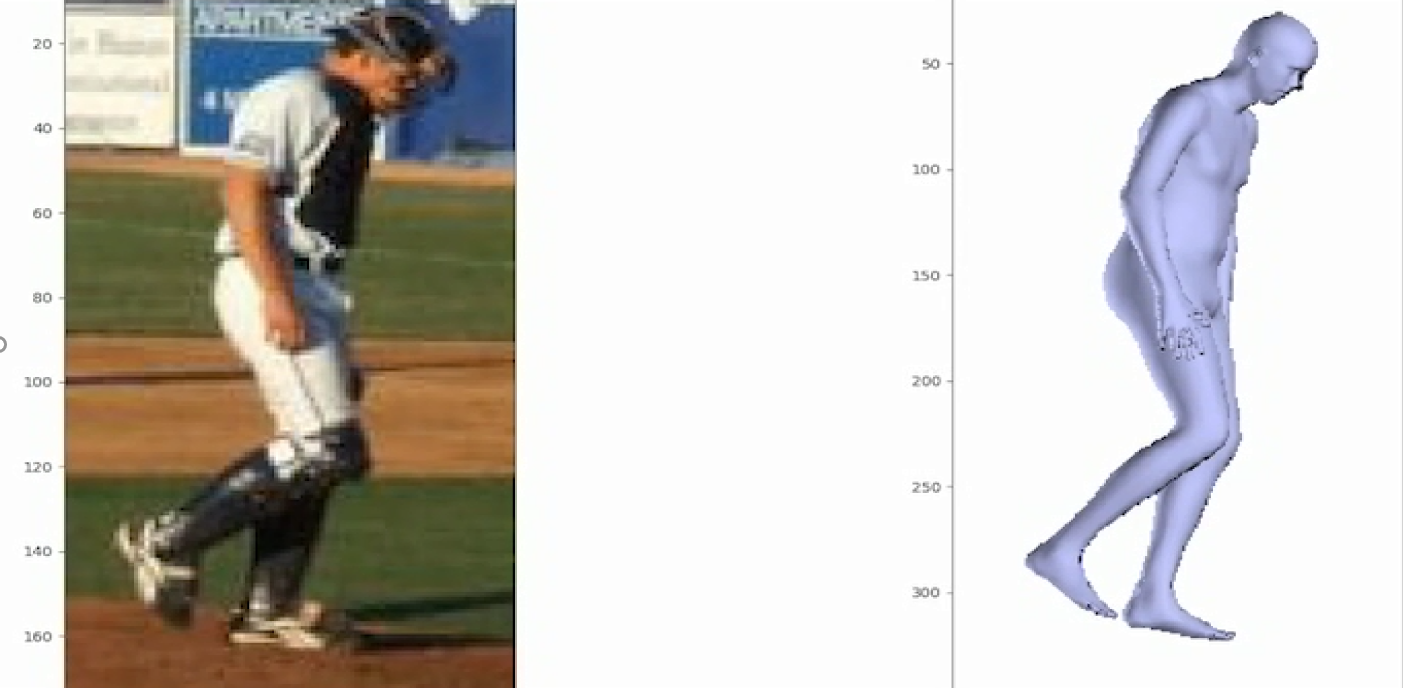
\includegraphics[width=0.95\linewidth]{fitting_smpl}}
        \caption{SMPLify: Fitting the SMPL model to the Leeds Sports Dataset.}
        \label{fig:smplify}
    \end{figure}
        
    \subsubsection{Direct regression}
    The most recent, and state-of-the-art approaches employ deep learning techniques to solve the entire optimization problem by directly regressing shape and pose parameters of the template model. An early approach by Tan et al.~\cite{tan17indirect} used deep neural networks to learn an encoding $f: \RR{H}{W} \mapsto (\pose, \shape, \trans, K)$ of input images to SMPL pose and shape, translation and camera parameters. Their method makes use of a \emph{silhouette renderer} $R : (V, T) \mapsto \{0,1\}^{H \times W}$ (learnt using synthetic data) capable of producing a binary silhouette from a predicted SMPL mesh. In this way, $R$ allows the network's SMPL predictions to be supervised to ensure generated silhouettes match ground-truth annotations. 
    Improvements were realised by incoporating an abudance of available human data into the training pipeline. Apart from 3D morphable models (e.g. SMPL~\cite{loper15smpl}), methods use paired 3D motion capture data (e.g. Human3.6M~\cite{ionescu2013human3,IonescuSminchisescu11}, 3DPW~\cite{vonmarcard2018recovering}) to help relate 2D appearance and the underlying 3D structure, unpaired 3D motion capture data (e.g. CMU~\lazycite{CMU}{CMU}) for learning detailed priors over the distribution of human shapes and poses, and large 2D keypoint datasets (e.g. MSCOCO~\lazycite{COCO}{COCO}, LSP~\lazycite{LSP}{LSP}, MPI~\lazycite{MPI}{MPI}) which help promote generalization to `in-the-wild' scenarios. A notable work in this category is Human Mesh Recovery (HMR) of Kanazawa et al.~\cite{kanazawa18end-to-end}, although multiple concurrent works exist\lazycite{https://proceedings.neurips.cc/paper/2017/file/ab452534c5ce28c4fbb0e102d4a4fb2e-Paper.pdf}{Hsiao-Yu Fish Tung}, \lazycite{https://www.seas.upenn.edu/~pavlakos/projects/humanshape/}{pavlakos}, \lazycite{http://virtualhumans.mpi-inf.mpg.de/papers/omran2018NBF/omran2018NBF.pdf}{neural body fitting} and \lazycite{DenseRaC}{DenseRaC}. Chapter 6 of this thesis will explore a method for modelling uncertainty in 3D reconstruction, by exploring extensions to the aforementioned architectures.

    % Show the basic structure of these networks in a picture
    
    BodyNet \lazycite{https://www.di.ens.fr/willow/research/bodynet/}{bodynet} follow a similar pipeline with the inclusion of a texture prediction module supervised by 2D body part segementations \lazycite{body part dataset}{dataset}. Silhouette data has also been shown to assist in accurate reconstruction of clothes, hair and other appearance detail~\cite{alldieck2019learning} \lazycite{https://arxiv.org/pdf/1901.00049.pdf}{SiCloPe} \lazycite{https://arxiv.org/abs/2004.04572}{ARCH}. Methods typically represent 3D clothes as `freeform' vertex deformations; in other words, deformations beyond the standard SMPL blend shapes which represent unclothed bodies. This presents significantly more degrees of freedom in the optimization, which must be controlled; either by large training datasets with limited variation or mesh-based deformation priors such as ARAP. 

    While the dominant paradigm in human reconstruction is now end-to-end deep learning methods, SPIN~\cite{kolotouros19learning} show impressive improvement by incorporating an energy minimization process within their training loop to further minimize a 2D reprojection loss subject to fixed pose \& shape priors. This idea inspired the work presented in Chapter 5 of this thesis, in which a 3D dog shape prior is learnt during the training loop via expectation maximization.

    % https://openaccess.thecvf.com/content_ICCV_2019/papers/Xu_DenseRaC_Joint_3D_Pose_and_Shape_Estimation_by_Dense_Render-and-Compare_ICCV_2019_paper.pdf
    
    There have also been a few recent works that reconstruct 3D humans without an explicit template prior. The general idea is to interpret a neural network as an implicit representation of the 3D surface. In particular, the network $f$ is trained to map sampled 3D locations $(x,y,z) \in \R{3}$ to an occupancy value $\{0,1\}$ (and optionally a texture value $(r,g,b) \in \R{3}$). This results in a memory efficient representation of the 3D surface as the space used to embed the surface does not need to be explicitly stored. Saito et al.~\cite{pifuSHNMKL19,saito2020pifuhd} present an example of such an architecture. Their network maps 3D locations with ResNet~\lazycite{Resnet}{Resnet} features sampled at coordinates projected with a known weak-perpective camera to occupancy and texture values. Li et al.\lazycite{https://project-splinter.github.io/monoport/}{MonoPort} later sped up reconstruction and rendering to allow real-time inference. Neural Radiance Fields (NeRF) capture high resolution details of static scenes by mapping 3D coordinates $(x,y,z)$ and viewing directions $(\theta, \phi)$ to volume density and view-dependent emitted radiances. The work was adapted to articulated structures~\lazycite{ANerf}{ANerf} by learning new skin for the SMPL model, using SPIN~\cite{kolotouros19learning} as a basic 3D skeleton predictor. A current downside of these techniques is the need to train a separate model per scene/subject and the slow inference time. However, these works do demonstrate high quality results and are a worthy direction for future research.

    % Show the basic structure of these networks in a picture

\subsection{Model-based animals}

    Having discussed reconstruction methods for other articulated subjects, this section will move on work related to the main topic of this thesis: 3D reconstruction of animal subjects. As summarized above, there are multiple challenges associated with animals which are not present with humans. Firstly, the general class of animal subjects is significantly more diverse in appearance and structure than the human category. This holds (although to a lesser extent) with various important animal subcategorizations, such as the class of medium-to-large quadrupeds, dog breeds, or birds. This diversity leads to challenges when designing 3D morphable models, since extreme deformations must allowed while penalizing even subtle adapations deemed unnatural. Also of concern are the significant variations in animal motion patterns (causing complex self-occlusion), body textures including fur (which vary even within breeds) and difficult environmental conditions. An interesting advantageous aspect to reconstructing animals is that they are less frequently clothed; a common nusiance factor for human reconstruction. These factors combined with practical challenges associated with capturing and annotating images has also led to a lack of open-source datasets which depict animal subjects. Of particular concern to this thesis is the lack of 3D training data captured from real animal subjects (typically using motion capture or static scans). Equivalent resources made available for humans have been used as a basis for building 3D morphable models (e.g. SMPL~\cite{loper15smpl}, FAUST~\lazycite{FAUST}{FAUST}), for learning priors over human shape and pose~\lazycite{learning priors}{learning priors}, and to provide per-image 3D supervisation when training deep neural networks~\cite{kanazawa18end-to-end}. Thankfully, online animal imagery which could serve as the basis for future datasets is plentiful, as are datasets with 2D silhouette data~\cite{lin2014microsoft,everingham2010pascal,DAVIS2017-2nd}. A formal comparison is given in \Cref{tab:animal-dsets}.  While animals are often featured in computer vision literature, there are still relatively few works that focus on accurate 3D animal reconstruction. However, the creative approaches used in these methods makes a formal review worthwhile. A summary of recent approaches is tabulated in \Cref{tab:literature}.
    
    % Please add the following required packages to your document preamble:
% \usepackage{booktabs}
\begin{table}[]
    \begin{tabular}{@{}lllll@{}}
    \toprule
    Dataset & Modality & Annotation & Subject & Num. Examples \\ 
    \midrule
    MSCOCO~\cite{lin2014microsoft} & Image (RGB) & S2, BB2 & DCaHoZSECoBG & 23,467 \\
    PascalVOC~\cite{everingham2010pascal} & Image (RGB) & S2, BB2 & xxx & xxx \\
    DAVIS~\cite{DAVIS2017-2nd} & Video (RGB) & S2 & xxx & xxx \\
    StanfordDogs & Image (RGB) & BB2 & D (120 breeds) & 20,580 \\
    \textbf{StanfordExtra} & Image (RGB) & J2, S2 & D (120 breeds) & 12,000 \\
    \textbf{BADJA} & Video (RGB) & J2, S2 & xxx & xxx \\
    AnimalPose & Image (RGB) & J2 & xxx & xxx \\
    SMAL & N/A & MM3 & DCaHoZCoTLHi & 47 \\
    \bottomrule
    \end{tabular}
    \caption{Dataset summary: analysis of available datasets. 
        Bold rows are datasets introduced in this thesis.
        S2: 2D Silhouettes, BB2: 2D bounding boxes, J2: 2D Joints, 
        MM3: 3D Morphable Model. P3: 3D Priors. M3: 3D Model.
        D: dog, Ca: cat, Ho: horse, Z: zebra, S: sheep, 
        E: elephant, Co: cow, B: bear, G: giraffe,
        T: tiger, L: lion: Ch: cheetah, Hi: hippo}
    \label{tab:animal-dsets}
\end{table}

% lin2014microsoft,everingham2010pascal,DAVIS2017-2nd

    

\newcommand{\awfhang}[1]{
    \begin{minipage}[t]{\textwidth}% Top-hanging minipage, will align on
                                   % bottom of first line
    \begin{tabbing} % tabbing so that minipage shrinks to fit
    \\[-\baselineskip] % Make first line zero-height
    #1 % Include user's text
    \end{tabbing}
    \end{minipage}} % can't allow } onto next line, as {WIDEBOX}~x will not tie.
    
    \newcolumntype{L}[1]{>{\RaggedRight\hspace{0pt}}p{#1}}
    \newcolumntype{R}[1]{>{\RaggedLeft\hspace{0pt}}p{#1}}
    
    \begin{table}[t!]
    {\sffamily
    \scriptsize
    \def\hd#1{\awfhang{#1}}
    \begin{tabular}{@{}L{20mm}%Paper
    |L{12mm}%Class
    L{15mm}%Train
    |L{15mm}%Template
    L{17mm}%Video
    L{17mm}%Test
    |L{9mm}%Model
    L{5mm}%Size
    @{}}
    \hd{Paper}%
    &\hd{Animal\\Class}%
    &\hd{Training\\requirements}%
    &\hd{Template\\Model}%
    &\hd{Video\\required}%
    &\hd{Test Time\\Annotation}%
    &\hd{Model\\Fitting}%
    &\hd{Test\\Size}%
    \\\hline
    %%%%%%%%%%%%%%%%%%%%%%
    This paper
    & Dogs  % 2D Joints, Silhouettes, 3D Template, 3D Priors
    & J2, S2, T3, P3
    & SMAL
    & No & None & No & 1703
    \\\hline
    %%%%%%%%%%%%%%%%%%%%%%
    3D-Safari~\cite{Zuffi19Safari}        
    & Zebras, horses
    % 3D models (albeit synthetic), 2D Joints,  Silhouettes,  3D Priors
    & M3 (albeit synthetic), J2, S2, P3
    & SMAL
    & 3-7 frames / animal & None & Yes & 200
    \\\hline
    %%%%%%%%%%%%%%%%%%%%%%
    Lions, Tigers and Bears (SMALR)~\cite{zuffi_lions} 
    & MLQ
    & Not trained
    & SMAL
    & 3-7 frames / animal & J2, S2 & Yes & 14
    \\\hline
    %%%%%%%%%%%%%%%%%%%%%%
    3D Menagerie (SMAL)~\cite{zuffi2017menagerie}                
    & MLQ 
    & Not trained
    & SMAL
    & No & J2, S2 & Yes & 48 
    \\\hline
    %%%%%%%%%%%%%%%%%%%%%%
    Creatures Great and SMAL~\cite{biggs2018creatures}
    & MLQ
    & Not trained
    & SMAL
    & Yes & S2 (for best results shown) & Yes & 9             \\\hline 
    %%%%%%%%%%%%%%%%%%%%%%
    Category Specific Mesh Reconstructions~\cite{kanazawa2018birds}
    & Birds
    & J2, S2
    & Bird convex hull
    & No & None & No & 2850          
    \\\hline
    %%%%%%%%%%%%%%%%%%%%%%
    What Shape are Dolphins~\cite{cashman2013shape}
    & Dolphins, Pigeons 
    & Not trained
    & Dolphin Template
    & 25 frames / category & J2, S2 & Yes & 25
    \\\hline
    %%%%%%%%%%%%%%%%%%%%%%
    Animated 3D Creatures~\cite{reinert2016animatedsketching}
    & MLQ
    & Not trained
    & Generalized Cylinders
    & Yes & J2, S2 & Yes & 15
    \\\hline
    \end{tabular}
    }
    \caption{Literature summary: Our paper extends large-scale ``in-the-wild'' reconstruction to the difficult class of diverse breeds of dogs. 
    MLQ: Medium-to-large quadrupeds. J2: 2D Joints. S2: 2D Silhouettes. T3: 3D Template. P3: 3D Priors. M3: 3D Model.}
    \label{tab:literature}
    % \vspace{-8mm}
    \end{table}
    
    

    % Table~\ref{tab:literature} summarizes previous work on animal reconstruction.
    % It is interesting to note that while several papers demonstrate reconstruction across species, which {\em prima facie} is a richer class than just dogs, the test-time requirements (e.g. manually-clicked keypoints/silhouette segmentations, input image quality etc.) are considerably higher for those systems.
    % Thus we claim that the achievement of reconstructing a full range of dog breeds, 
    % with variable fur length, varying shape and pose of ears, and with considerable occlusion, is a significant contribution.

    % \subsubsection{Animals intro}

    % Cashman and Fitzgibbon~\cite{cashman2013shape} obtained one of the first 3D morphable animal models, but their work was limited to small classes of objects (e.g. dolphins, pigeons), and did not incorporate a skeleton.  Their work also showed the use of the 2D silhouette for fitting, which is key to our method. 
    % Reinert {\em et al.} \cite{reinert2016animated} meanwhile construct 3D meshes by fitting generalized cylinders to hand-drawn skeletons.
    % Combined skeletal and morphable models were used by Khamis {\em et al.}~\cite{hand-shape} for modelling the human hand, and Loper {\em et al.}~\cite{loper15smpl} in the SMPL model which has been extensively used for human tracking. 

    % The SMPL model was extended to animals by Zuffi {\em et al.}~\cite{zuffi2017menagerie}, where the lack of motion capture data for animal subjects is cleverly overcome by building the model from $41$ 3D scans of toy figurines from five quadruped families in arbitrary poses. Their paper demonstrates single-frame fits of their model to real-world animal data, showing that despite the model being built from ``artists' impressions'' it remains an accurate model of real animals. This is borne out further by our work.  Their paper did however depend on per-frame human annotated keypoint labels, which would be costly and challenging to obtain for large video sequences. This work was recently extended~\cite{zuffi_lions} with a refinement step that optimizes over model vertex positions. This can be considered independent to the initial SMAL model fit and would be trivial to add to our method.

    % \subsubsection{Learning animal shape from unrelated 2D images}
    % Early work in reconstructing animals includes Chen et al.~\lazycite{chensharks}{chensharks} who learn a simple shape space by registering 11 3D shark models. 
    Early work in animals focuses on learning 3D animal shape spaces by registering an input 3D model to image collections. Examples include Chen et al.\lazycite{chensharks}{chensharks} who learn a shark model and Cashman et al.~\cite{cashman2013shape} who recover a parameterized, morphable 3D model from unrelated 2D images depicting examples of the target class. Their method requires user-supplied 2D object outlines and point constraints for each image, and a single rigid mesh for the entire object class. The authors demonstrate recovering an 8-parameter morphable dolphin model from 32 images sourced from the Internet. To reduce required user activity, it is reasonable to assume that given sufficient labelled training data, it would be simple to manipulate a convolutional network architecture able to perform foreground / background segmentation and identify key points (say, joints) for the desired object class. The system achieves impressive results when optimizing over both pose and shape parameters across a range of object classes, but suffers from an overly smooth shape representation which causes trouble for strongly articulated classes such as polar bears.

    \begin{figure}[H] % Example image
        \center{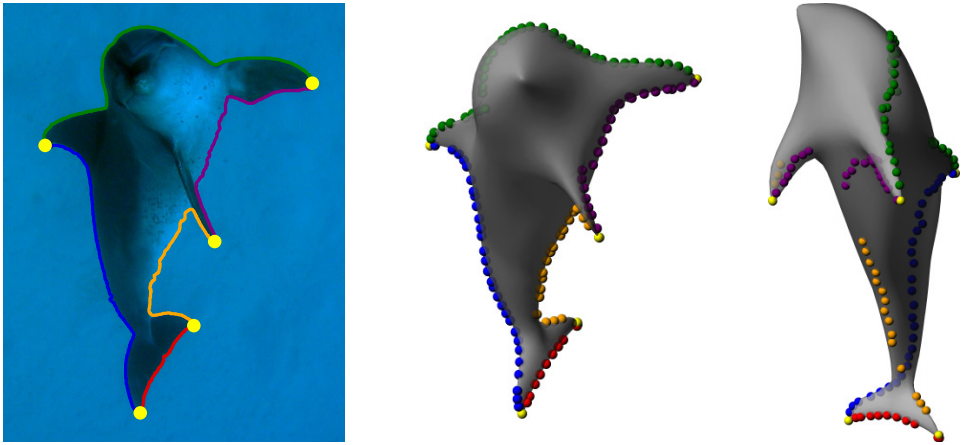
\includegraphics[width=0.7\linewidth]{dolphins}}
        \caption{8-parameter dolphin model with annotated contour (left) and contour generators (middle and right).}
        \label{fig:cashman_fitzgibbon}
    \end{figure}

    % \subsubsection{Fitting to animal video sequences (Stebbing)}

    The approach was later extended to articulated classes in work by Stebbing et al.~\cite{arap_stebbing}, who optimize a 3D template model to animal video sequences. In this work, rather than defining an inner skeleton, the template model is rigged with virtual markers, which assign each mesh vertex $v_i$ to one of $M$ groups that share a set of basis rotations $B_{m}$. User interaction is again reuqired to segement the animal from the background and to provide mesh-to-image keypoint correspondences.

    \begin{figure}[H]
        \centering
        \begin{subfigure}{0.5\textwidth}
        \centering
            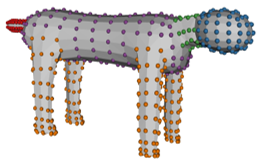
\includegraphics[height=0.5\linewidth]{arapsfm/arap_annotated_template}
            \caption{Template mesh with joint movement constraints.}
        \end{subfigure}%
        \begin{subfigure}{0.5\textwidth}
        \centering
            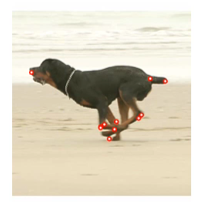
\includegraphics[height=0.5\linewidth]{arapsfm/arap_point_tracks}
            \caption{Example of user supplied point tracks.}
        \end{subfigure}%
        \caption{User input required for the deformable mesh animation algorithm, reprinted from~\cite{arap_stebbing}.}
        \label{fig:arap_user}
    \end{figure} 

    Through reasonably accurate pose fitting and by allowing some pose-invariant shape deformation, this work produces smooth meshes which match the input video. Moreover, experimentation demonstrates that ARAP is a useful prior for reconstructing articulated, non-rigid motion in instances that an internal skeleton is a priori unknown. However, the shape attributes for the reconstructed model are not particularly accurate, which results in frequent errors appearing at internal occluding contours. In addition, the large non-convex optimization algorithm is an expensive operation, taking around 1 minute per video frame on a standard Linux workstation. Results are shown on 11 sequences.

    Results showing this work fitting a crude dog template mesh to a sample video obtained from YouTube are shown previously in Figure \ref{fig:intro_arap_output}. Figure \ref{fig:arap_output} shows another example, which operates on a template impala mesh.

    \begin{figure}[H]
        \center{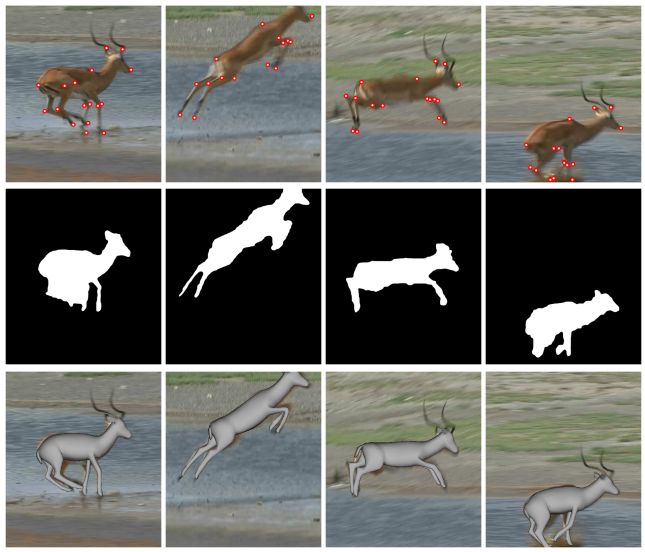
\includegraphics[width=0.95\linewidth]{arapsfm/arap_impala}}
        \caption{Example of an impala template being fit to input video sequence, reprinted from~\cite{arap_stebbing}}
        \label{fig:arap_output}
    \end{figure}

    Related is the work of Ntouskos et al.\lazycite{ntouskos}{ntouskos} who use an optimization scheme to combine geometric primitives fit to segmented animal parts. Favreau et al.~\lazycite{favreau}{favreau} follow a similar approach, fitting geometric primitives to a 2D video sequence with manually sketched body part labels. 

    \subsubsection{Fitting the SMAL mesh to animal images}
    % Draw out the silhouette term as important here
    % Talk about subsequent SMALR + SMALST in the same section
    Unfortunately, none of the techniques above are suitable for reconstructing an animal category with significant shape diversity.     Zuffi et al.~\cite{zuffi2017menagerie} made a significant contribution by releasing SMAL, a deformable 3D quadruped model (analagous to SMPL~\cite{loper15smpl} for human reconstruction) build from $41$ scans of artist-designed toy figurines. The authors also released shape and pose priors generated from artist data. The authors also discuss a small modification to the SMPLify~\lazycite{smplify}{smplify} approach in order to fit the SMAL model to RGB animal input images. However, an example result showing the result of the optimizer fitting the SMAL mesh to an RGB image of a fox can be seen in Figure \ref{fig:smalify}. The whole optimization process takes around 1 minute per frame. 

    \begin{figure}[H] % Example image
        \center{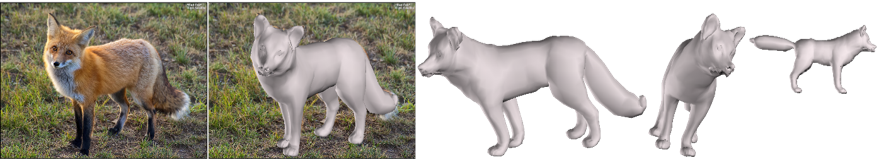
\includegraphics[width=0.95\linewidth]{fitting_smal}}
        \caption{Fitting SMAL to a hand segmented animal, reprinted from~\cite{zuffi2017menagerie}.}
        \label{fig:smalify}
    \end{figure}

    The terms of the optimization largely mirror the work of SMALify, although the interpenetration term is ommited and joints are provided manually rather than by a CNN. Importantly, the optimization incoporates an additional \emph{silhouette} term which aligns the 3D model shape to a binary silhouette image extracted by a user. Chapter 4 of this thesis shows silhouette terms are of particular importance when reconstructing accurate animal shape. The following definition describes the process for differentiably rendering a 3D model to form a silhouette image which can then be compared to the provided 2D silhouette:

    \begin{definition}[Differentiable Rendering]
        The process of generating a 2D image from a 3D polygon mesh is known as rendering and can be achieved through a process known as raytracing. Raytracing is a rendering technique able to generate photorealistic 2D images from the scene. It can be considered the opposite process by which the human eye perceives the world, as this method involves lines being cast outwards, beginning at a point known as the \emph{camera origin}. Figure \ref{fig:raycasting} shows a typical set up, in which rays are cast from the camera origin through each pixel on the image plane. The colour for the pixel is obtained by following the ray through the scene until a light source or non-reflective surface is reached, taking into account any reflections or non-opaque scene items. Due to the considerable comptuation required, the operation is often parallelized and assigned to the GPU. However, the technique is typically considered unsuitable for real-time rendering of complex scenes (due to complex ray paths) or when high resolution images (many rays required) are needed. However, for this work, scenes are typically made up of a single non-reflective, solid mesh surface and contain no complex elements (e.g.\ shadows, non-constant lighting.

        \begin{figure}[H] % Example image
            \center{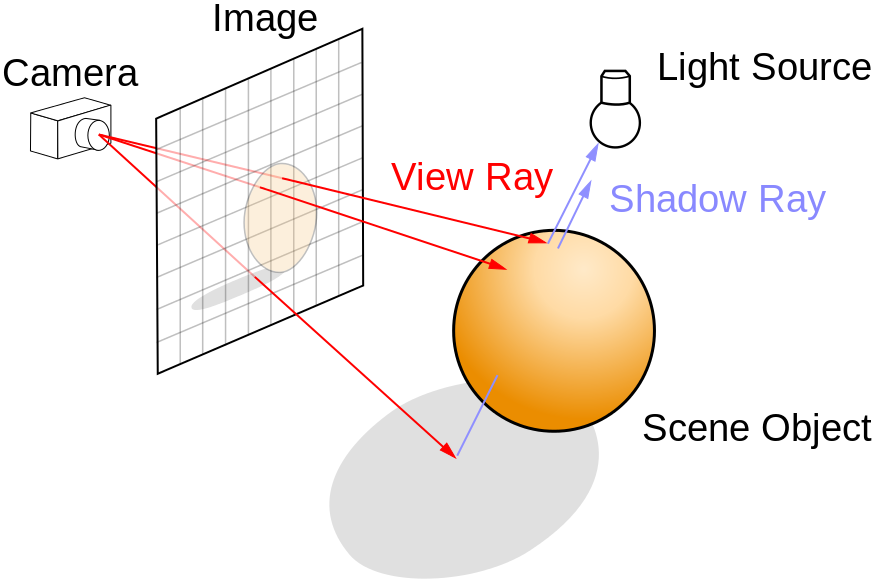
\includegraphics[width=0.5\linewidth]{ray_trace}}
            \caption{Diagram showing raycast rendering.~\cite{rendering}.}
            \label{fig:raycasting}
        \end{figure}

        It is also worth noting that the standard method for raycasting is not differentiable, causing problems for differentiable optimizers (including neural networks). However, alternative rendering methods~\cite{loper2014opendr} are available for these purposes.
    \end{definition}

    The SMAL authors~\cite{zuffi2017menagerie} demonstrate their system by fitting their deformable 3D model to quadruped species. Subsequent work includes SMALR~\cite{zuffi_lions}, who fit to multiple images of an animal and incoporate similar freeform deformation term used to model clothing in 3D human pipelines. They show their technique, which takes advantage of multi-view constraints afforded by fitting to video sequences, allows high-quality reconstructions of more exotic animal categories with details not covered in the original SMAL 3D model training set. 
    
    A common property of techniques discussed so far is the reliance on manual annotations (commonly 2D silhouettes and keypoint correspondences) at test time. 3D-Safari~\cite{Zuffi19Safari} overcome this by training a deep network on synthetic data (generated by applying SMALR~\cite{zuffi_lions} on a large input dataset) to recover detailed zebra shapes in the wild. Chapter 4 of this thesis demonstrates a technique which overcomes the need for a large input dataset of joint annotations by training on synthetic data generated from the graphics model alone. 
    
    A further drawback of the approaches is their reliance on a test-time energy-based optimization procedure, which is susceptible to failure with poor quality keypoint/silhouette predictions and increases the computational burden. Chapter 5 of this method presents an automatic reconstruction method that overcomes the need for additional energy-based refinement, and is trained purely from single in-the-wild images. 
    
    Tangential to these approaches is the work of Kulkarni et al.\lazycite{Canonical Surface Mapping}{Canonical Surface Mapping} who reconstruct pose (although not shape) parameters for an rigged mesh using a deep network, learning from geometry cycle consistency terms rather than annotated keypoints. However, the shape is fixed to the input mesh and pose is also often confused, particularly determining the difference between the legs. The results appear of significantly poorer quality than the work in Chapter 5 of this thesis. Also of consideration is the end-to-end network of Kanazawa et al.~\cite{kanazawa2018birds} and subsequent paper which overcomes the need for keypoints by capturing uncertainty in camera viewpoints. In addition, their network does not require an input 3D morphable model, although they do initialize a sphere model to a mean bird. In addition, the bird category exhibits more limited articulation than our dog category. 
    
    
    % TODO:
    %Finally, there are techniques which do not produce a mesh~\cite{Agudo_2018_CVPR,novotny19c3dpo} or rely heavily on input 2D keypoints or video at test-time~\cite{vicente_3dv,Probst2018_ECCVa}.
    % Unsupervised Learning of Probably Symmetric Deformable 3D Objects from Images in the Wild
    % Canonical Surface Mapping via Geometric Cycle Consistency https://arxiv.org/abs/1907.10043



% \subsubsection{Literature review tables}

% The closest work in terms of scale is the category-specific mesh reconstruction of Kanazawa et al.~\cite{kanazawa2018birds}, where 2850 images of birds were reconstructed.  However doing so for the complex pose and shape variations of dogs required the advances described in this paper.




% \section{Model-free methods for non-rigid reconstruction}

\subsection{Shape-from-X}

\subsubsection*{Shape from silhouette.} Silhouette images have been shown to contain sufficient shape information to enable their use in many 3D recovery pipelines. Chen {\em et al.}~\cite{chen2010inferring} demonstrate single-view shape reconstruction from such input for general object classes, by building a shape space model from 3D samples. More related to our work, Favreau {\em et al.}~\cite{favreau2004animal} apply PCA to silhouette images to extract animal gaits from video sequences. The task of predicting silhouette images from 2D input has been effectively used as a proxy for regressing 3D model parameters for humans~\cite{tan17indirect,kanazawa18end-to-end} and other 3D objects~\cite{wiles2017silnet}.


% https://arxiv.org/pdf/1903.00812.pdf



% large dataset on large large Techniques in this section typically achieve this using data-driven machine learning algorithms, which can be trained on various  general, data-driven machine learning algorithms are used to predict an association between image pixels and locations with a semantic meaning. techniques used to achieve this techniques achieve this In general, data driven machine learning techniques are used to train an algorithm to associate image appearance features with semantically-meaningful partsIn order to teach a system to understand semantic this section, we will discuss techniques for predicting keypoints from a pre-defined list

% These approaches do offer some advantages; in particular, the approaches do not require a training procedure based on a labelled dataset, although the techniques cannot be used to associate image points to a representative 3D mesh. In this section, we will discuss techniques for predicting points from a pre-defined list 

% a labelled dataset this does offer some advantages (particularly that the approaches do not require a labelled dataset for training, data 

% and in general, the number of correspondences the number of detected correspondences can differ between test examples and there is no pre-determined there is no pre-determined list of detected correspondences points the methods should obtain, and in general the number of returned keypoints can differ  used for identifying 2D image points based on a pre-defined   approach to identifying image points, although this time the desired locations will are pre-defined.

% \begin{enumerate}
%     \item Talk about all 2D keypoint detection techniques
%     \item Talk about 
% \end{enumerate}

% For example, For example, techniques such as SIFT generate different feature descriptions for two points taken on different zebras, due to the different patterns. Such systems also struggle greatly under object-viewpoint, particularly for 

% which relies on local gradient information will generate different feature descriptions for two points taken on different zebra since the patterns may differ. The next class of techniques are designed to overcome this limitation, and offer matching based on \emph{semantic point correspondences}.




% unfortunately, these techniques 

% such as to ensure uniqueness ensure specificity and comparing feature descriptors computed from them. Early feature descriptors focus only Feature descriptors often capture local statistics related to the image location and aim to have some invariance to different lighting conditions, scales, rotations or other transforms. from which  (typically repeatible features such as edges Techniques fall into two categories: global image descriptors are calculated on the whole image, and have some advantages in that they are invariant to matching based on the whole image, and have some advantages since they are naturall invariant to invarient 

% majority of techniques solve matching based on local image-features, techniques match based on local features, i.e. rely on general, techniques are used to identify so-called \emph{interest points} which have some repeatibility properties for which a \emph{feature descriptor} can be Historically, the most successful methods operate by Early techniques designed for stereo matching and for optical flow were designed to operate under small viewpoint changes, but early technique proved suitable for stereo matching under small viewpoint changes, but was not rotation invariant and for deriving point correspondences since the 1980s, echniques for deriving point correspondences between images has existed since the 1980soperated on image pixel intensity values, without much consideration for the underlying objects. Improvements were made with geometric techniques, such as edge and corner detectors, which offered some robustness to varying lighting conditions. However, the mid-level features represenations of SIFT~\cite{}, HOG~\cite{}, DAISY~\cite{}, VLAD~\cite{} etc. offered considerable improvements, allowing point matching under various object scales and camera viewpoints.

% However, while suitable for processing such techniques were unfortunately unable to match semantically-meaningful keypoint locations across different object instances

% the feature representations of techniques struggle with varying camera viewpoints, still typically fail when 

% at some robustness to that related mid-level appearance features, such as corners 

% Major imawithout consideration for the objects they purely on image pixels, with little knowledge of the objects they Of course, determine which 2D image locations are in correspondence 

% The history of deriving point correspondences begins with stereo and optical flow, which use 

% Even the earliest reconstruction techniques, such as in stereo or optical flow based methods, rely on point correspondences to determine 3D structure. 

% to use of point correspondences to 


% For example, imagine we have captured multiple images ${I_1, I_2, ...}$ of the same static scene containing a dog. A classical approach for recovering the 3D 3D dog For example, imagine we have various images captured of the same static scene containing a dog. In order to determine the consider a real-world point on the end of a dog's nose for which we have yet to determine the true 3D world location. To recover the 3D point, we may start by grouping together projections of this point $\{(u_i, v_i)\} \in R^2$ in various images we have captured of the scene. From these point correspondences, we could begin 


% we may start We may start by grouping together various projections of this point in various images we have captured of the scene From various images captured of the scene, we may start by grouping together the various projections of this nose point it is useful to group together the various projections of this point . Further, we can various projections of this point in on the end of a dogs nose, scene containing a dog, we can group to group 2D image points 

% points a scene containing a dog, we may wish to group , whether in related locations between two images, an image and a 3D surface or two 3D surfaces. Often, point correspondences are used to group together multiple image views of the same real-world location, or to relate an image point with a location on a representative 3D surface. 


% Throughout the long history of 3D reconstruction, nearly all methods which focus on recovering complex 3D objects from 2D image data make use of \emph{point correspondences} to constrain the problem. By understanding which pairs of Early work focuses on \emph{image matching} to 


% In order to reconstruct a complex 3D object from 2D image data, we typically require significant constraints from Techniques which reconstruct complex 3D subjects from 2D image data typically require 

% In order to reconstruct a complex 3D subject from 2D image data, it is almost always essential to constrain  3D articulated subject from 2D image data, it is almost always image, it is alms3D reconstruction has a long history 3D reconstruction techniques have a long history in reconstruction, and nearly all require as 

% \begin{enumerate}
%     \item 3D reconstruction techniques rely upon point correspondences. This has a very long history:
%     \item Optical flow, mid-level discriptors (SIFT, DAISY etc.)
%     \item More recently, pose estimation techniques have found themselves useful 
% \end{enumerate}




% \section{Obtaining animal test data}
%     A significant drawback due to the lack of available training data is that state-of-the-art segmentation pipelines require a wealth of (RGB Input, Segmentation) and (IR Input, Segmentation training pairs which are not readily available for animal targets. To resolve this, a collaborative project is underway between GSK and Texuna to design a bespoke camera module which can be fit into rodent, dog, mini-pig and rabbit enclosures. Figure \ref{fig:texuna_cage} shows a recent prototype design. The cameras are able to flip between RGB and IR capture modes and use IP camera technology, which is supported by a number of off-the-shelf recording systems. Once animal data is successfully recorded, it will be passed to human annotators to create a suitable dataset to train a segmentation network. Until this has been obtained, the system is designed on the premise of receiving perfect silhouette segmentations. 

%     % Talk a little more about the data -- problems (all outside?), occlusions, pets, number of pictures per animal (distribution) 
%     For testing, there are examples of real-world animal segmentations that form a satisfactory set for system testing. Between the Weizmann Horse Dataset~\cite{weizmann}, the IIIT-OXFORD PET dataset~\cite{oxfordpetdata} and animal superclasses from popular datasets such as MS Coco~\cite{lin2014microsoft} and PASCAL VOC~\cite{everingham2010pascal}, there are approximately one thousand RGB-segmentation pairs for independent images (i.e.\ not part of an available video sequence). It is worth noting that the distribution of images is heavily weighted towards cats, dogs and horses over other animal species. Moreover, images tend to be taken in outdoor environments with side-on animal views. This bias has been partially resolved by sourcing an additional 1500 frames from YouTube and the BBC Blue Planet II documentary series\footnote{Appropriate permissions have been sought where applicable}. These sequences were all segmented by hand, using the RotoBrush tool provided by the Adobe After-Effects~\cite{Bai:2009:VSC} package.  









